 % scopiazzato dal template di Matteo Longeri (grazie!)
%%%%%%%%%%%%%%%%%%%%%%%%%%%%%%%%%%%%%%%%%%%%%%%%%%%%%%
\documentclass[12pt,a4paper]{report}
% o article, book, ...
%%%%%%%%%%%%%%%%%%%%%%%%%%%%%%%%%%%%%%%%%%%%%%%%%%%%%%
% packages...
\usepackage[utf8]{inputenc}
\usepackage[english,italian]{babel}
\usepackage[hyphens]{url}
\usepackage{wrapfig}


\usepackage{hyperref}
\usepackage{graphicx}
\usepackage{paralist}
% Per inserire testo a caso in attesa di realizzare i capitoli
\usepackage{lipsum}
\usepackage{todonotes}
\usepackage{setspace}

\onehalfspace %per interlinea da 1.5

\newcommand{\datiAnalisi}{\url{https://doi.org/10.5281/zenodo.3612806}}
\newcommand{\datiQuestionari}{\url{https://doi.org/10.5281/zenodo.3627829}}
\newcommand{\urlRepoSW}{\url{https://github.com/simoneScaravati/Physiradio}}

\newcommand{\physiradio}{Physiradio} %decidiamo se camel case o no

\usepackage{array}
\newcolumntype{P}[1]{>{\centering\arraybackslash}p{#1}} %per precisione nelle tabelle
\newcolumntype{M}[1]{>{\centering\arraybackslash}m{#1}}

\usepackage{multirow}
\usepackage{float}

%per codici sia bash che c++
\usepackage{xcolor}
\definecolor{commentgreen}{RGB}{2,112,10}
\definecolor{eminence}{RGB}{108,48,130}
\definecolor{weborange}{RGB}{255,165,0}
\definecolor{frenchplum}{RGB}{129,20,83}
\usepackage{listings}
\usepackage{textcomp}

\lstdefinestyle{customBash}{
	language=bash,
	frame=tb, 
	tabsize=4,
	basicstyle=\small\ttfamily,
	showstringspaces=false,
	commentstyle=\color{red},
	keywordstyle=\color{blue}
}


\lstdefinestyle{customC++Arduino}{
	language=C++,
	frame=tb,
	tabsize=4,
	showstringspaces=false,
	numbers=left,
	upquote=true,
	commentstyle=\color{commentgreen},
	keywordstyle=\color{eminence},
	stringstyle=\color{red},
	basicstyle=\footnotesize\ttfamily, % basic font setting
	emph={int,char,double,float,unsigned,void,bool},
	emphstyle={\color{blue}},
	%escapechar=\&,
	% keyword highlighting
	classoffset=1, % starting new class
	morekeywords={>,<,.,;,,,-,!,=,~},
	keywordstyle=\color{weborange},
	classoffset=0,
}

%\lstset{language=bash,frame=tb}
%\lstset{language=C++,frame=tb}

%per riquadro
\usepackage[linewidth=1pt]{mdframed}

% Per generare il file PDF aderente alle specifiche PDF/A-1b. Verificarne poi la validità.
\usepackage[a-1b]{pdfx}
%\usepackage[pdfa]{hyperref}
%%%%%%%%%%%%%%%%%%%%%%%%%%%%%%%%%%%%%%%%%%%%%%%%%%%%%
\begin{document}

% Frontespizio
\begin{titlepage}
\begin{center}

\includegraphics[width=\textwidth]{Immagini/Logo.jpg}\\
{\large{\bf Corso di Laurea Triennale in Informatica}}
\end{center}
\vspace{12mm}
\begin{center}
{\huge{\bf Physiradio:}}\\
\vspace{4mm}
{\huge{\bf Uno studio sulla Data}}\\
\vspace{4mm}
{\huge{\bf Physicalization tramite lo}}\\
\vspace{3mm} %non lo so perchè ma così è dritto
{\huge{\bf sviluppo di un device IoT}}\\

\end{center}
\vspace{14mm}
\begin{flushright}
{\large{\bf Tesi di Laurea di:}}\\
{\large{\bf Simone Scaravati}}\\
{\large{\bf Matr. 870883}}\\
\end{flushright}
\vspace{8mm}
\begin{flushleft}
{\large{\bf Relatore:}}\\
{\large{\bf Prof. Andrea Trentini}}\\

\end{flushleft}
\vspace{16mm}
\begin{center}
{\large{\bf Anno Accademico 2019-2020}}
\end{center}
\end{titlepage}

\tableofcontents
% o sections (dipende dal documentclass)

%\listoftodos
%\todo{i termini stranieri in corsivo, a parte quelli proprio dati per italianizzati come file}
%\todo{atrent: fonte immagine, su tutte}

\chapter{Introduzione}

La Data Physicalization è stata definita come 
\begin{quote}
``\emph{Un'area di ricerca che esamina in quale modo, le rappresentazioni fisiche dei dati, supportate da computer, possano aiutare la cognizione, la comunicazione, l'apprendimento, il \textit{problem-solving} e \textit{il decision making} }'' \cite{jansen2015opportunities}
\end{quote} %\todo{simo to atrent: esiste un modo carino in italiano per dirlo? atrent: va bene anche così, in corsivo}

Nel corso degli anni, grazie alla pervasività, e alla differenziazione, delle tecnologie che ognuno di noi ha a disposizione, la rappresentazione dei dati ha assunto un ruolo sempre più importante in diversi campi di ricerca, come l'informatica, l'educazione o la comunicazione.\\ 
La \textit{data physicalization}, essendo un'area di ricerca molto recente, sta acquisendo sempre più rilevanza in questi campi. Questo la porta ad essere aperta a nuove idee e spunti per essere arricchita ed ampliata, portando a sperimentare nuovi modi per poter rappresentare dei dati, di varia natura, attraverso metodi non convenzionali e che, rendendoli tangibili, non sfruttino solamente la vista come mezzo di cognizione ed interpretazione del dato.\\


Il lavoro svolto in questa tesi, è stato quello di studiare i vari aspetti riguardanti la ``fisicalizzazione'' dei dati, e ha portato conseguentemente allo sviluppo di un prototipo che potesse presentare uno spunto interessante per la \textit{data physicalization}.
Nello specifico si tratta di un device IoT, che prende il nome di \physiradio, il quale riproduce specifici flussi musicali secondo una mappatura che trasla le condizioni meteorologiche, accessibili tramite API aperte (open data), in generi musicali e colori; processo che viene nominato \textit{musicalization}.\\
L'obiettivo principale di questo esperimento è verificare se un tale dispositivo può essere uno spunto per aumentare la curiosità sul mondo della \textit{data physicalization}, dei dati aperti, e in secondo luogo verificare se il genere musicale può essere utilizzato in una mappatura dei dati. Quest'ultima fase è stata eseguita tramite un \textit{field testing}, dove il prototipo è stato sottoposto ad un gruppo di utenti, che hanno compilato un questionario, da cui è stato possibile estrarre dati utili all'analisi dell'efficacia del device e della curiosità generata.


\section{Data Physicalization}\label{sec:dataphys}

La \textit{data physicalization}, che nel corso di questo elaborato verrà a volte tradotta (senza alcun riferimento a lavori altrui) in ``fisicalizzazione dei dati'', è un'area di ricerca multidisciplinare moderna, basata sulla rappresentazione fisica di dati, di qualsiasi natura e tipo. \\
Le rappresentazioni dei dati tramite supporti fisici esistono da secoli, ricercabili persino nell'antichità. Ad esempio nella Figura \ref{fig:mesopotamiantokens} possiamo osservare come già nella Mesopotamia del 5500 a.c., venissero utilizzati oggetti di varia natura (denominati successivamente, dagli archeologi, ``token''\cite{mesopotamianTokens}), con un ordine ben specifico, per avere un'idea chiara e immediata del conteggio di merci o tasse.


\begin{figure}
	\begin{center}
		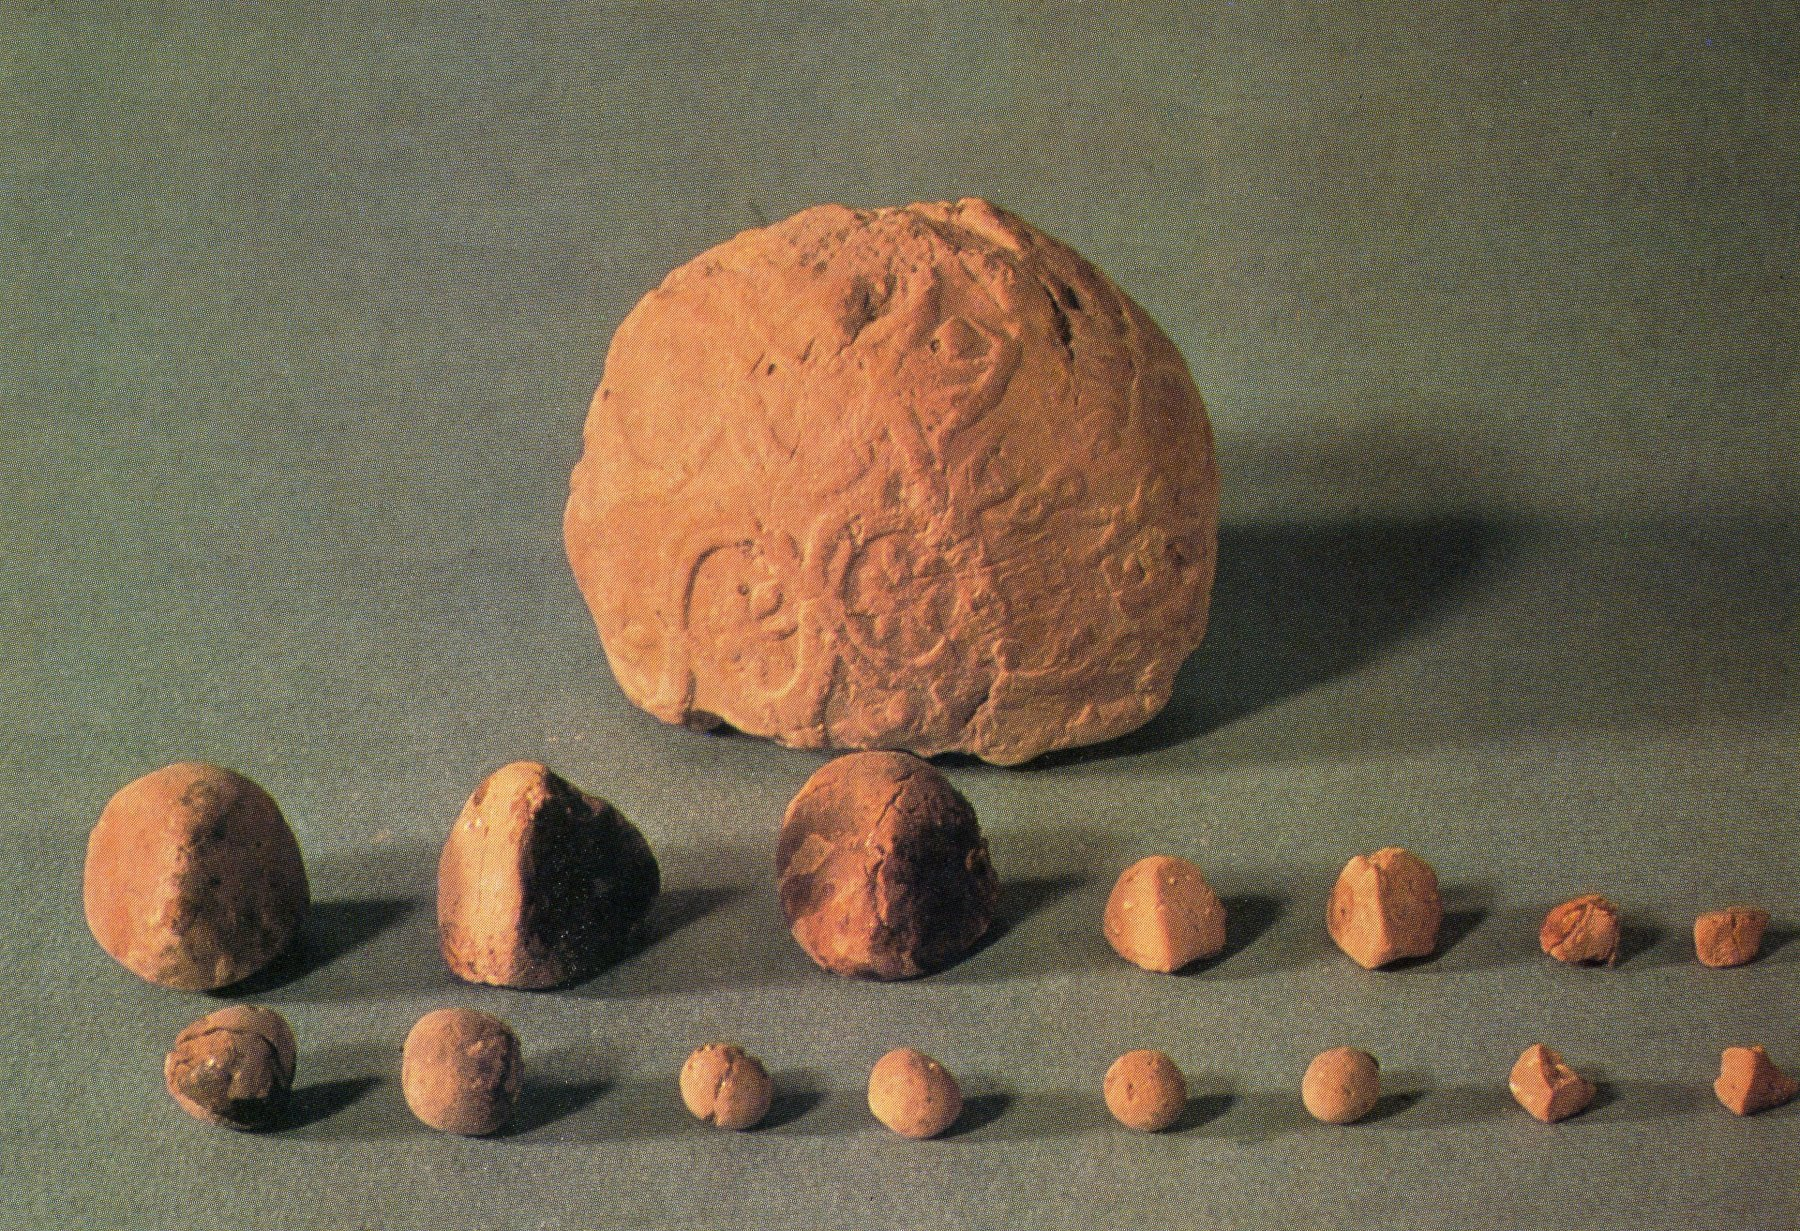
\includegraphics[scale=0.7]{Immagini/mesopotamian_tokens.jpg}
		\caption{Token mesopotamici, fonte \cite{mesopotamianTokens}}
		\label{fig:mesopotamiantokens}
	\end{center}
\end{figure}


Come questo esempio, ce ne sono molti altri, consultabili sul sito ufficiale dedicato alla \textit{data physicalization} \cite{dataphys_org_list}, gestita da Yvonne Jansen, che  è la referente principale a livello internazionale per quanto riguarda questa branca di ricerca.\\ 

Entrando nello specifico della fisicalizzazione dei dati. Essa potrebbe essere confusa con la \textit{data visualization}, ovvero la mera visualizzazione dei dati, cosa a cui tutti noi siamo abituati quotidianamente, basti pensare a quanti grafici, animazioni e numeri vediamo ogni giorno sui nostri smartphone o computer. In effetti, entrambe si riferiscono a modi per rappresentare dei dati. La \textit{data visualization} cerca un modo di comunicare i dati attraverso l'uso di una mappatura sistematica tra segni grafici e valori dei dati nella creazione della visualizzazione. Questa mappatura stabilisce come i valori dei dati verranno rappresentati visivamente, determinando come e in che misura una proprietà di un segno grafico, come la dimensione o il colore, cambierà per riflettere le variazioni del valore di un dato.\\
Partendo da questo concetto, la \textit{data physicalization} si spinge oltre\cite{jansen2015opportunities}, domandandosi se esistano altri tipi di rappresentazioni, che non si limitino solamente alla raffigurazione grafica. \\
Il punto chiave insita nel fatto che, nelle visualizzazioni, viene sfruttata solamente la vista come mezzo di trasmissione e cognizione dell'informazione, mentre potrebbe essere ancora più utile e di maggiore interesse cercare di sfruttare anche altri sensi del corpo umano.\\
A tal proposito, si possono citare Emerge \cite{emergePhysicalPlot} e TastyBeats \cite{tastybeats} (Figura \ref{fig:examples_other_phys}). Il primo è un insieme di barrette posizionate verticalmente, sopra un sistema di pistoni motorizzati, che permettono di vedere e interagire, tramite quindi l'uso della vista e del tatto, con dei dataset di varia natura. Il secondo invece, consta di un sistema di piccole pompe idrauliche, tramite cui è possibile creare un energy drink le cui componenti variano dinamicamente a seconda degli allenamenti fisici che vengono svolti, rappresentando di conseguenza dati relativi ad attività motorie attraverso il gusto.\\


\begin{figure}
	\begin{center}
		\centerline
		{
			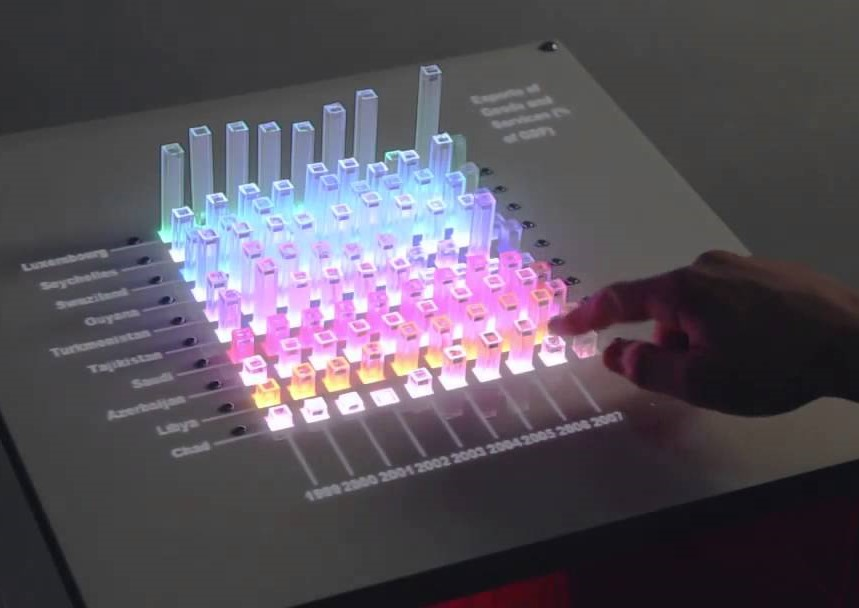
\includegraphics[width=.400\textwidth]{Immagini/emergePhysicalPlots.jpg}
			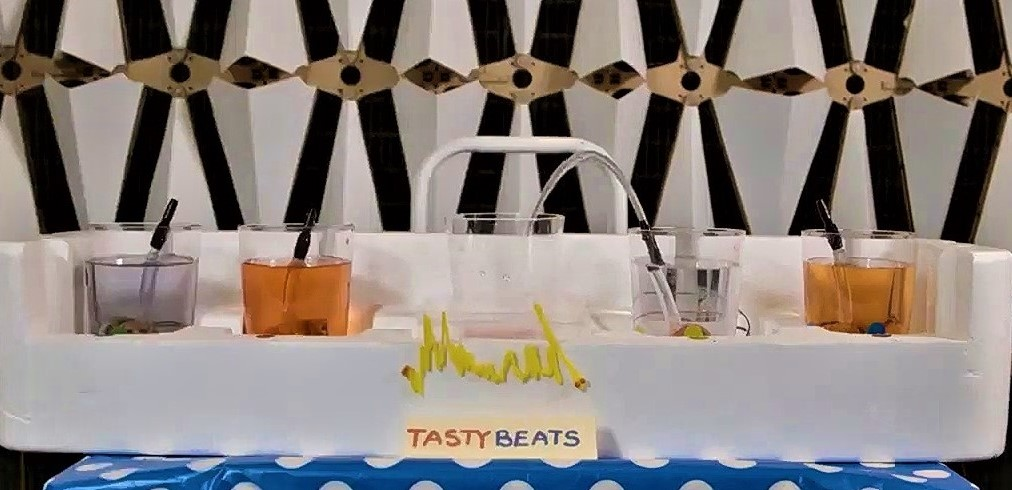
\includegraphics[width=.585\textwidth]{Immagini/tastybeats.jpg}			
		}
		\caption{Esempi di \textit{data physicalization}. Emerge (sinistra) e TastyBeats (destra), fonti \cite{emergePhysicalPlot} e \cite{tastybeats}}
		\label{fig:examples_other_phys}
	\end{center}
\end{figure}
%\todo{simo to atrent: immagini superflue? atrent: ma no lascia}


Le recenti creazioni di interfacce tangibili, tecnologie pervasive avanzate e la distribuzione sempre più diffusa di sistemi e componenti integrati, hanno portato allo sviluppo di creazioni ``moderne'' per rappresentare i dati, attraverso strumenti informatici associati a sensori, attuatori, ecc\dots\ , che permettono di avere rappresentazioni di carattere dinamico e interattivo; caratteristiche non molto presenti in progetti sviluppati precedentemente.\\ %\todo{simo to atrent : so che è debole}

Secondo \cite{jansen2015opportunities} la \textit{data physicalization} può:
\begin{compactitem}
	\item ``Aiutare le persone a esplorare, comprendere e comunicare i dati, utilizzando le rappresentazioni fisiche, basate sui computer, dei dati'';
	\item Rendere i dati più accessibili/raggiungibili a tutti;
	\item Favorire benefici cognitivi;
	\item Democratizzare i dati nel mondo reale;
	\item Coinvolgere le persone.
\end{compactitem}

L'aspetto della democratizzazione è proposto anche in \cite{verweij2019domestic} dove i ``widget domestici" vengono utilizzati per supportare con successo la creatività domestica e la co-creazione delle rappresentazioni di dati.

In \cite{tanenbaum2013democratizing} ``DIY, hacking and craft" sono suggeriti come potenti strumenti di democratizzazione. I dispositivi IoT (Internet of Things) sono sfruttati in \cite{houben2016physikit} in riferimento a ``Il potenziale per democratizzare l'accesso, l'uso, e appropriazione dei dati'', poiché ``la maggior parte dei dati è una `scatola nera' in natura: gli utenti spesso non sanno come accedere ai dati o interpretarli''. Questi dispositivi ``integrati nelle case", possono essere utilizzati per coinvolgere utenti non tecnici, il che è stato uno spunto importante per lo sviluppo del prototipo.\\

Può la creazione di un dispositivo fisico familiare e non minaccioso (ad esempio una radio dall'aspetto vintage) essere un veicolo di trasferimento delle conoscenze? Potrebbe, un oggetto del genere, essere in grado di suscitare curiosità sulla fonte e la disponibilità di alcuni dati (ad esempio il meteo atmosferico) e le tecniche alla base dell'accesso, dell'estrazione e dell'analisi dei dati?
%I lavori precedenti sono promettenti.
%\todo{atrent: ultima frase stona in italiano. simo: finire con una domanda è peggio?}


\section{Analisi degli studi}\label{sec:analisistudi}

Il primo step del lavoro è stato di quello di effettuare un'analisi della \textit{state of the art}. %\todo{simo to atrent: si traduce in italiano solitamente? atrent: puoi lasciarla in inglese (corsivo) o mettere semplicemente "analisi della bibliografia"}.
In particolare, si è scelto di focalizzarsi sui paper riguardanti prototipi/prodotti fisici effettivamente funzionanti, che potessero conferire una reale implementazione del concetto di \textit{data physicalization}, incentrandosi sul tipo di messaggio che viene trasportato e tramite quali sensi.\\
Come fonte principale dell'analisi, è stata utilizzata la lista di documenti elencati nella bibliografia del sito ufficiale per la \textit{data physicalization} \cite{dataphys_org_bib}.\\
Sono stati analizzati tre principali fattori per ogni prototipo/progetto presentato:
\begin{enumerate}
	\item Quali sensi umani sono stati sfruttati
	\item Il livello di interazione con l'oggetto
	\item Il livello di dinamicità dei dati
\end{enumerate}

\medskip
Riguardo all'analisi svolta: sebbene vi sia una consapevolezza sul fatto che questa analisi possa essere soggettiva, in riferimento all'atto di leggere e interpretare gli articoli, si è cercato di renderla il più ``meccanica” possibile, adottando i seguenti criteri:

\begin{compactenum}
	\item SENSES: valore booleano per indicare quali sensi sono stati sfruttati (SIGHT=vista, TOUCH=tatto, HEARING=udito, TASTE=gusto, SMELL=olfatto) dove $1=$ il senso è stato sfruttato e $0=$ il senso non è stato sfruttato.
	\item INTERACTION: il livello di interazione da parte dell'utente con l'oggetto, espresso con tre valori numerici interi distinti:
	\begin{compactitem} 
		\item $0 =$ nessuna interazione, la creazione si limita ad essere osservata.
		\item $1 =$ l'interazione col prototipo cambia i parametri di fisicalizzazione, cioè come vengono rappresentati i dati, ma questi ultimi rimangono invariati.
		\item $2 =$ l'interazione col prototipo cambia anche il dataset di riferimento.
		
	\end{compactitem}
	
	\item DYNAMICITY: flag booleano tradotto in STATIC(falso/0) e DYNAMIC(vero/1), dove DYNAMIC indica che vi è una costante connessione tra il device e i dati, ovvero che se i dati cambiano, cambia anche la fisicalizzazione (\textit{real time}). STATIC indica che i dati di riferimento sono statici. 
\end{compactenum}


Da questa analisi è stato prodotto un dataset, pubblicato su Zenodo\cite{datiAnalisi}, da cui è possibile estrarre informazioni utili. \\
I risultati (Figura \ref{fig:tablesenses}) mostrano che i sensi più utilizzati sono la vista e il tatto; mentre l'udito, il gusto e l'olfatto vengono raramente sfruttati. \\
Questo è stato uno spunto molto importante per la realizzazione del device, perché ci si è chiesto se esistesse un modo per trarre vantaggio da questi sensi ``minori''. \\
Riconoscendo le difficoltà tecnologiche e creative nello sfruttare l'olfatto e il gusto come sensi per una fisicalizzazione, il senso rimanente era l'udito: in questo modo nacque l'idea di usare la musica come mezzo di comunicazione del dato. \\%e il genere in particolare.
In effetti, la musica fa parte della vita di tutti: lo si voglia o meno, tutti noi la ascoltiamo. Ed essa riesce a stimolare emozioni e stati d'animo, che possono essere utili per canalizzare dei dati. Sebbene la percezione di ogni canzone, di qualsiasi genere e artista, sia diversa per ognuno di noi, il pensiero di usare la musica come mezzo per fisicalizzare i dati, ovviamente attraverso l'udito, era convincente.\\

Naturalmente, la musica può portare soggettività nell'interpretazione e introduce diversi problemi nella classificazione, dovuti a diverse variabili. Tuttavia, lo scopo principale del device non sarà quello di creare il miglior modo in assoluto per poter fisicalizzare dei dati, ma sarà quello di proporre una soluzione che stimoli la curiosità degli utenti. Di conseguenza, anche se il metodo utilizzato per la \textit{physicalization} non sarà perfetto, comunque potrebbe essere sufficientemente valido per il suo scopo.\\

Successivamente, sono stati considerati gli altri due fattori: l'interattività con gli oggetti e la dinamicità dei dati usati dai dispositivi. L'analisi dei documenti, mostra livelli bassi (Figura \ref{fig:interacivityandcuriosity}) per entrambi gli aspetti. La maggior parte dei dispositivi utilizza dati statici (circa l'80\%), mentre l'interazione fisica con l'oggetto risulta spesso inesistente e si limita alla mera osservazione(interazione$ = 0$ in circa il 57\% dei casi), il 23\% propone un primo livello di interazione e solo il restante 20\% presenta un'interazione tale da riuscire a cambiare i dati alla fonte. \\
Pertanto, partendo dai risultati di questa ricerca, per la creazione del device si è optato per una soluzione in grado di gestire i dati in tempo reale (quindi dinamici), e dove l'esperienza di interazione con esso sia concreta, tale che non ci si limiti solamente ad osservare il dispositivo.

\begin{figure}
	\begin{center}
		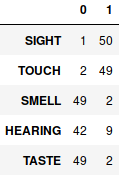
\includegraphics[scale=0.9]{Immagini/ENG_tableSenses.png}
		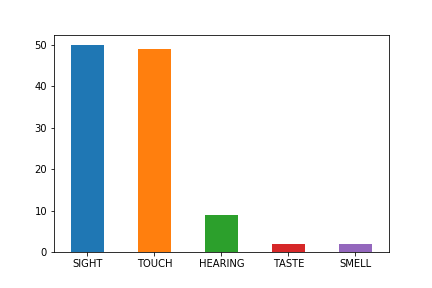
\includegraphics[scale=0.40]{Immagini/ENG_barplot_1.png}
		\caption{Sensi utilizzati nei dispositivi analizzati inerenti alla \textit{Data Physicalization}. Casi totali: 51}
		\label{fig:tablesenses}
	\end{center}
\end{figure}

\begin{figure}
	\begin{center}
		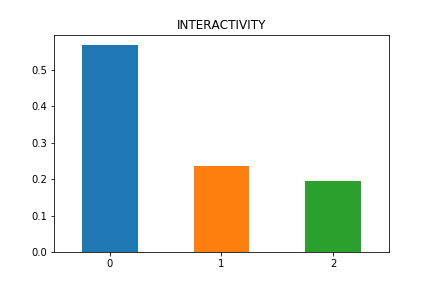
\includegraphics[scale=0.4]{Immagini/ENG_interactivity.png}
		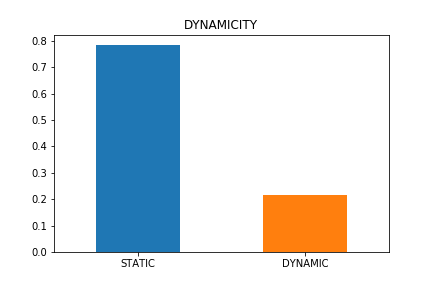
\includegraphics[scale=0.4]{Immagini/ENG_dynamic.png}
		\caption{Livelli di interattività con i device e dinamicità dei dati. Casi totali: 51}
		\label{fig:interacivityandcuriosity}
	\end{center}
\end{figure}

In seguito sono stati individuati due punti critici per la creazione del device: quali dati usare e come usarli in funzione alla musica. \\

Vedremo nei prossimi capitoli come, per il primo caso, ci si sia indirizzati verso il mondo dei dati aperti, per aumentare ulteriormente il grado di curiosità dell'esperienza e per cercare di avvicinare, al mondo della fruizione dei dati liberi, anche i non addetti al settore.\\
Per il secondo punto invece, l'utilizzo della musica si focalizzerà sull'utilizzare i generi musicali per eseguire la mappatura dei dati per la \textit{physicalization}. Si elencheranno i pregi e i difetti di questa scelta, e il perché è stata presa.



\section{Open Data}\label{sec:opendata}

%questo era l' intro
%I dati aperti sono un concetto tecnico e un movimento politico poiché i set di dati (sull'ambiente, le imprese, ecc.) Possono essere utilizzati per verificare / falsificare le politiche governative (ex ante ed ex post) ("responsabilità civile"). Ma l'analisi dei dati non è per le masse: il cittadino medio potrebbe non conoscere nemmeno l'esistenza di dati aperti. Qui la sfida è suscitare interesse, curiosità e necessità per conoscenza nella persona comune. La fisicizzazione dei dati può essere di qualche aiuto: creando un dispositivo familiare (ad esempio una radio) che "materializza" alcuni dati disponibili al pubblico, gli autori stanno cercando di aumentare la curiosità sulla fonte e la disponibilità di dati aperti (ad es.
%stato meteorologico) e le tecniche alla base dell'accesso, dell'estrazione e dell'analisi dei dati.



Gli open data sono diventati un movimento mondiale che coinvolge attori governativi e non governativi.
La Open Knowledge Foundation (OKF, \cite{okd}) è stata una delle prime organizzazioni a definire ``apertura'' in questo contesto, la sua definizione può essere citata come: ``Dei dati sono aperti se qualcuno è libero di usarli, riutilizzarli e ridistribuirli, con al più l'attribuzione della creazione'' (vale a dire che i dati possono essere utilizzati apertamente in termini di licenze). %\todo{atrent: traduzione automatica non riletta ;)}
Il ``HM Government’s Open Data White Paper'' \cite{HMgov} afferma che il Open Government Data consta di ``Informazioni del settore pubblico che sono state rese disponibili al pubblico come dati aperti '' e definisce le Informazioni del Settore Pubblico (PSI) come ``dati e informazioni prodotti, raccolti o detenuti da autorità pubbliche, nell'ambito del loro compito pubblico'', dati che dovrebbero essere accessibili (idealmente via Internet) a costi marginali (se non nulli) e senza discriminazioni, disponibili in un formato digitale e leggibile da una macchina, e fornito senza restrizioni sull'uso o sulla ridistribuzione.


%Berners-Lee \cite{5starsOD} e Davies \cite{davies2010open} hanno definito le valutazioni dei dati aperti, per evidenziare l'importanza degli aspetti tecnici dell'apertura, ad esempio attraverso l'uso di standard aperti e formati di file non proprietari per la pubblicazione di dati aperti.
%Inoltre, Berners-Lee e altri autori \cite{govdata, bizer2009linked} hanno promosso il concetto di `` dati aperti collegati '' per trasformare `` dati sul web '' in `` rete di dati '' incoraggiando il collegamento dei propri dati con altri dataset. \todo{simo to atrent: questa parte non mi piace proprio, la salto per ora}


Gli open data sono un concetto tecnico, il quale sta anche diventando rilevante dal punto di vista politico, poiché i dataset (su ambiente, imprese, ecc\dots) possono essere utilizzati per verificare o falsificare le politiche governative (\textit{ex ante} ed \textit{ex post}): i dati aperti possono essere un mezzo per la ``responsabilità civica''. %\todo{civica}
Qualsiasi cittadino, con sufficiente conoscenza, è in grado di recuperare dati (che possono essere ritenuti più affidabili se provengono da fonti di terze parti) da server pubblici e studiare l'effetto di leggi come, ad esempio, un cambiamento della tassazione del tabacco sul numero di fumatori, il divieto di alcuni tipi di veicoli in base alla qualità dell'aria \cite{trentini2014lombardy}, l'introduzione di una legislazione specifica per ridurre il numero di persone disoccupate, ecc\dots\ \\


Tuttavia, ``l'analisi dei dati non è per le masse'' \cite{puussaar2018making}: il cittadino medio non è a conoscenza dell'esistenza di dati aperti e/o non è in grado di estrarre informazioni da un dataset. \\

Considerando gli obiettivi del device che verrà creato, ossia aumentare l'interesse e la curiosità nel fruitore sulla fisicalizzazione di un dato, il fatto di poter usufruire di dati aperti e liberi può essere un valore aggiunto, specialmente per i non addetti ai lavori.\\ 
Anche se alla fine l'utente deciderà di non imparare come analizzare i set di dati, almeno avrà avuto la possibilità di ragionare sull'occasione di sfruttare il suo diritto alla ``responsabilità civica", con l'aiuto di una persona specializzata, o un oggetto, che gli permetta farlo al posto suo; strumenti come \physiradio\ sarebbero molto calzanti.


%\subsection{Esempi di dataset}

%\todo{simo to atrent : in realtá non farei un capitolo a sè stante, lo metterei sempre dentro gli open data ma come esempi, perché di fatto la data physicalization non punta solo ai dataset. 
%atrent: e a cosa d'altro? 
%simo: i dati meteo stessi non sono una mera collezione di dati (non con una definizione standard del termine per lo meno, con cui ci si riferisce a dati strutturati in forma relazionale), e di esempi di fisicalizzazioni che non usano dei dataset ce ne sono un po'. e tra l'altro, se mi focalizzo sui dataset poi sembra meno credibile la scelta dei dati meteo}


\subsection{OpenWeatherMap e la scelta delle condizioni meteorologiche}\label{sec:openweather}

Una volta analizzati gli open data e le loro potenzialità, ci si è chiesto quali dati effettivamente prelevare.\\
Il problema maggiore era legato al fatto che, per un primo prototipo da sviluppare, era necessario scegliere dei dati aperti che fossero di facile comprensione, per avere un esempio di funzionamento intuitivo anche da persone non provenienti da studi scientifici/tecnici.\\

Dopo alcune ricerche e analisi, le condizioni meteorologiche sono risultate la scelta più naturale e utile allo scopo, perché sono qualcosa alla portata di tutti e di cognizione immediata.\\
Per quanto possano sembrare un'informazione inutile\footnote{Citando Robin Williams nel film ``Good Morning Vietnam": ``Com'è il tempo? Hai una finestra? Aprila!''}, tuttavia, nel contesto di questo esperimento, è stato un buon punto di partenza per conversazioni e stimoli a suggerimenti che sono arrivati da parte degli utenti (vedere nelle conclusioni, sezione \ref{sec:conclusions}). Inoltre, come vedremo nei capitoli successivi (legati ai software implementati), comunque il prototipo non si limiterà a descrivere il tempo di una sola città, ma è comunque interrogabile per analizzare tutte le città registrate nei server della piattaforma utilizzata.\\

Si è deciso così che \physiradio\ si basi su OpenWeatherMap\cite{openWeather}, una piattaforma di dati aperta che fornisce molti servizi meteorologici. Per interagire con i suoi dati, essa fornisce delle API (Application Programming Interface) di tipo REST, che consentono l'accesso, via software, ai dati meteorologici in tempo reale.\\
In particolare, i dati restituiti sono sotto forma di file JSON, il che è molto utile: non solo sono di facile interpretazione da parte di moltissimi sistemi, ma numerosi dataset di open data utilizzano questo formato. Questo implica che \physiradio\ potrà essere agevolmente modificato/migliorato per sviluppi futuri, sfruttando altri dati da rappresentare. 


\section{``Musicalization'': il processo di physicalization tramite la musica}\label{sec:musicalization}

Successivamente, ci si è concentrati sull'utilizzo della musica come mezzo principale per questo esperimento di \textit{data physicalization}.\\

La musica è un mondo molto vasto, con una semantica tutta propria, complessa ed articolata. Essa può trasmettere una vasta gamma di emozioni, sentimenti e stati d'animo. Quando si tenta di analizzare un brano, ci sono molti parametri da considerare: tempo (bpm), modo (maggiore/minore), \textit{pitch}, \textit{loudness}, ecc\dots\ Inoltre, è complicato valutare quale canzone è più adatta ad un particolare contesto come presentato in \cite{han2010music}, dove viene descritto un approccio alla musica rispetto alla classificazione delle emozioni.
Un altro aspetto fondamentale è che i testi di una canzone possono trasmettere informazioni all'ascoltatore (se le parole sono comprese, ovviamente), ma la musica e i testi possono essere discordanti per l'umore che la canzone vuole canalizzare\footnote{ad esempio, ``Some Nights" dei Fun è famosa per questa caratteristica, avendo un arrangiamento musicale dai toni allegri e vivaci, mentre il testo narra di tragedie avvenute in tempi di guerra.}, %\todo{simo to atrent: meglio come footnote questa? atrent: mah in generale alcune footnote del testo potrebbero essere portate inline, in questo caso invece ok footnote} 
causando problemi a qualsiasi sforzo di classificazione.\\

Considerando tutti questi aspetti della musica, è evidente che vi sono delle difficoltà non irrilevanti nel tentativo di creare una classificazione tale che sia percepita in maniera totalmente oggettiva e uguale da tutti. Tuttavia, prendendo atto che l'obiettivo principale dell'esperimento non è quello di creare un mapping perfetto, si è deciso di perseguire comunque questa strada, adottando i criteri che seguono.\\

Esistono tecniche specifiche per trasferire informazioni tramite la semplice generazione di singoli suoni, come la cosiddetta \textit{sonificazione} \cite{sonificationNasaUrl}. Abbiamo degli esempi in \cite{bonafede2018proposal} e \cite{ludovico2016sonification}, dove vengono presentate tecniche di tracciamento del volto e di sintesi del suono per ``sonificare'' le espressioni facciali al fine di aiutare le persone con problemi visivi e un sistema di riferimento per interpretare modelli già esistenti di sonificazione e propone modelli futuri.\\
Un suono semplice e costante, però, non può essere ascoltato per un lungo periodo di tempo, perché può risultare molto fastidioso. Di conseguenza, quando si deve usare una tecnica più morbida e sopportabile (per l'ascoltatore), entra in gioco la \textit{musificazione}.\\
La musificazione è stata definita come la rappresentazione musicale dei dati. È pensata per andare oltre la sonificazione diretta: essa include elementi di tonalità e l'uso di scale modali per costruire composizioni musicali (vedere \cite{sonificationMusification}), che generano strutture musicali (spartiti) con delle caratteristiche di livello superiore, come la polifonia o la modulazione tonale, per intrattenere l'ascoltatore di più, e per più tempo, rispetto al caso della sonificazione.\\

La musificazione e la sonificazione hanno una caratteristica in comune, ovvero il fatto di essere deterministici nei risultati: dato lo stesso input, l'output, sia esso un suono, uno spartito o una traccia musicale, sarà sempre lo stesso. Questo determinismo può risultare a sua volta ``noioso'', se applicato in un contesto di vita quotidiana.\\
\physiradio\ cerca di ridurre al minimo questa potenziale sensazione di noia, ampliando l'associazione ``dato $\rightarrow$ musica'' introducendo l'idea di \textit{``musicalizzazione''}; il termine è stato introdotto in questa tesi senza alcun riferimento a lavori altrui.
Invece di generare suoni/musica ex novo, \physiradio\ sceglie e riproduce flussi musicali in streaming disponibili sulla rete, i quali sono etichettati in base al genere musicale (maggiori dettagli a riguardo nella sezione \ref{sec:mapping}).
In sostanza, il termine musicalizzazione si riferisce all'associazione tra valori di dati e brani musicali, che cambiano nel tempo, introducendo nel sistema un grado (potenzialmente alto, a seconda del flusso) di non-determinismo ``anti-noia''.


\subsection{Aggiunta del colore alla fisicalizzazione}\label{sec:colors}
%\todo{simo to atrent: un sotto capitolo è eccessivo per questa parte? atrent: no, però farei uno sforzo ulteriore per motivare introduzione colore visto che è stata criticata dai reviewer. simo: ho cercato di stare low profile perché in fase di testing abbiamo detto che si vedeva poco e certi utenti non ci facevano neanche caso. comunque ho cercato di ampliare - atrent:ok}
%\todo {atrent: su questo stare il più basso profilo possibile, anche perché nel prototipo la luce si vede poco (e molti manco la notano)}

Durante lo sviluppo del prototipo, analizzando lavori fatti da altri studenti/ricercatori, è stato pensato di aggiungere un altro senso sfruttato dalla fisicalizzazione, ossia la vista. La sua introduzione è dovuta a molteplici fattori: in primis, parliamo del senso più comunemente usato nella rappresentazione dei dati (come anticipato nella sezione \ref{sec:analisistudi}), dovuto anche alla vasta presenza delle \textit{visualization} in molti contesti a cui noi tutti siamo abituati. Di conseguenza l'utente medio è più abituato, molto probabilmente, a ricorrere alla vista, rispetto ad altri sensi, nelle prime fasi di interpretazione di qualsiasi dato. In secondo luogo, la vista, è stata ritenuta un utile sostegno all'udito perché, con una giusta legenda/didascalia (o comunque una conoscenza pregressa del mapping), rende più veloce ed intuitiva l'associazione del dato. % al genere musicale.
Perciò questo fattore, combinato con i generi musicali, potrebbe portare semantica e aiutare l'utente ad interagire meglio con il dispositivo, nell'interpretazione dei dati, aumentandone la leggibilità.\\ 

Per inserire la vista come ulteriore senso impiegato da \physiradio\ si è scelto di sfruttare i colori, in particolare una striscia di LED RGB che emette un singolo specifico colore che, a seconda della condizione atmosferica trovata, in combinazione con uno specifico genere musicale, formano una coppia ben precisa di dati, usata nel mapping (paragrafo \ref{sec:mapping}).\\
Per introdurre i colori, è stato fatto affidamento sul modello di Robert Plutchick \cite{plutchik2001nature}, in particolare è stata presa come riferimento la sua `ruota delle emozioni' (Figura \ref{fig:wheel_of_emotions}), perché è considerato uno dei più importanti studi psicologici sulle emozioni umane mappate sui colori. In combinazione con \cite{predictingmoodonmusicgenre}, uno studio che propone un abbinamento tra emozioni (\textit{mood} nello specifico) e generi musicali, crea la giusta base per poter sviluppare un mapping adeguato per il nostro device IoT. 

%\todo{simo to atrent: una parte di mapping l'ho introdotta qui perché mi sembrava necessario, va spostata sotto o va bene qui? atrent: ok qui}


\begin{figure}
	\begin{center}
		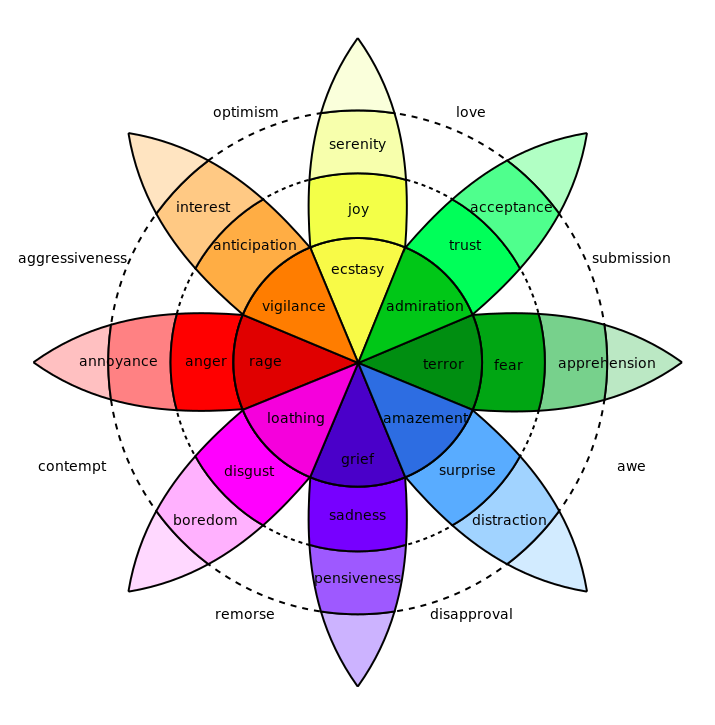
\includegraphics[width=.5\textwidth]{../TesiScaravati/Paper_ensemble_notes_and_tables/Plutchik-wheel.png}
		\caption{Ruota delle emozioni di Plutchik, fonte \cite{wheelofemotions}}
		\label{fig:wheel_of_emotions}
	\end{center}
\end{figure}


\section{Il mapping attuato}\label{sec:mapping}

Una volta prese le scelte riguardo a quali dati fisicalizzare (tempo atmosferico) e come fisicalizzarli (generi musicali e colori), si è dovuta affrontare la problematica del mapping da utilizzare.\\  
Lo schema di funzionamento di \physiradio\ è il seguente: ottiene i valori delle condizioni meteorologiche (tramite le API di OpenWeatherMap) di una città configurata via software, li elabora estraendo solamente la descrizione principale e il livello di umidità relativa, quindi li mappa su una combinazione di genere musicale e colore. La funzione di mappatura è così fatta:

\begin{center}
	$map(Descrizione\ Condizioni\ Metereologiche, Umidit \grave{a} \ relativa) \rightarrow (Genere\ musicale, Colore)$
\end{center}

Di seguito, vengono spiegate le motivazioni principali del perché sono stati scelti questi valori.\\

Il concetto base da cui si è partiti, è stato quello di avere come filo conduttore tra tempo atmosferico (umidità inclusa), genere musicali e colori, le emozioni/\textit{mood} che ognuno di essi poteva scaturire nell'utente medio. Di conseguenza, ci si é indirizzati verso lavori che cercassero una corrispondenza con le emozioni per ognuno dei tre componenti.\\
Per implementare questa funzione di mappatura sperimentale, è stato esaminato uno studio di riferimento \cite{karmaker2015automated}. In esso viene descritto il modello di un selettore musicale basato sulle condizioni meteorologiche, che è ciò che più si avvicina al device che si è voluto implementare. Nello specifico vengono presi in considerazione molti parametri sia per quanto riguarda la musica, che per il tempo atmosferico: per la prima si considerano modo, tempo, tonalità, ritmo, armonia e dinamica; mentre si considerano temperatura, umidità, pressione, vento, sole, nuvolosità e precipitazioni per il tempo atmosferico.\\
Tuttavia, per la funzione di mapping implementata da \physiradio\ è molto difficile, se non impossibile, tenere in considerazione tutti questi fattori. Per giunta non è questo il fulcro della ricerca, avendo come obiettivo quello di aumentare la curiosità sulla \textit{data physicalization} e sui dati aperti tramite un device IoT \textit{user friendly}, non è necessario avere un mapping perfetto. Si è dovuta perciò effettuare un scrematura.\\
Per il tempo atmosferico, oltre alla descrizione della condizione corrente, si è considerato unicamente il valore dell'umidità relativa, poiché era l'unico valore estraibile che potesse essere utile a livello ``superficiale'' (inteso come immediatezza di ricezione da parte dell'utente), come descritto in \cite{humiditylevel}, si è deciso di settare una soglia tale per cui il livello di umidità rende confortevole o meno il clima, in particolare si è deciso di applicare questa soglia ai tempi atmosferici `Sereno' (soleggiato piacevole contro afa) e `Pioggia/Pioggerella' (pioggia leggera contro pioggia abbondante). Basandosi sia sull'articolo poc'anzi citato che su test empirici, si è deciso di settare questa soglia a 85\% di umidità relativa.\\

Per quanto riguarda la musica invece, una prima implementazioni si era pensata tramite l'utilizzo di app di streaming musicali (come Spotify o Apple Music) per poter avere una scelta specifica delle tracce da selezioni (con un tagging potenzialmente maggiore). Tuttavia, ovviamente, quei servizi a pagamento non permettono di accedere direttamente a flussi audio per ovvi motivi commerciali. \\
Di conseguenza si è dovuti ripiegare su una soluzione effettivamente implementabile. La scelta è ricaduta sui generi musicali come macro classificazione per la ``musicalizzazione'', poiché vengono usati streaming di web radio liberamente utilizzabili, alcune delle quali sono estremamente selettive nel catalogo musicale (ci sono stazione che trasmettono solo Classica, altre solo Metal, ecc\dots), perciò permettono effettivamente di fare una selezione per genere.\\

La scelta dei colori invece come anticipato nella sezione precedente \ref{sec:colors}, si basa sullo studio delle emozioni di Plutchick\cite{plutchik2001nature}. \\
Per conciliare genere musicali e colori, e quindi ottenere la coppia di valori usata nella funzione di mapping, i mezzi utilizzati sono appunto il \textit{mood} e le emozioni che entrambi trasmettono all'uomo. Studi precedenti, come \cite{predictingmoodonmusicgenre}, analizzano come i generi musicali ispirino stati d'animo specifici alle persone.\\

Ciò nonostante, nello sviluppo del prototipo, sono stati necessari alcuni interventi, soggettivi e scarsi di fonti, riguardo alla scelta dei generi musicali usati. \\
In generale, i generi musicali moderni, come LoFi, ChillOut, Smooth Jazz e vari tipi di metal estremo, non sono stati menzionati in precedenti lavori accademici, tra quelli trovati ed esaminati durante lo svolgimento di questo studio. Tuttavia, questi generi si ritiene che siano molto suggestivi ed estremamente specifici: la maggior parte delle canzoni appartenenti a quei generi suoneranno molto simili tra loro, il che è utile se vogliono trasmettere le stesse informazioni ma con canzoni diverse.\\

Di conseguenza, qui di seguito, vengono riportati i principali criteri per poter associare i tempi atmosferici a determinati generi musicali.  In particolare, vi sono due casi di condizioni atmosferiche che sono stati implementati secondo criteri personali:
Il primo riguarda la condizione ``Neve'', la quale sembrava utile e funzionale, quasi in modo naturale, rappresentarla con canzoni natalizie, sebbene sia ovvio che non esista un \textit{mood} specifico legato alle ``festività natalizie''.\\
Il secondo, di spettro più ampio, è collegato a condizioni meteorologiche pericolose, come ``Tempolare'', `` Tornado '' oppure ``Acquazzone'', che possono, secondo un criterio puramente soggettivo, essere rappresentate con canzoni appartenenti al genere `Metal estremo', perché si è pensato che fosse il genere più appropriato per definire una situazione caotica e pericolosa, e molte canzoni appartenenti a questo genere sono davvero simili tra loro.\\
Per quanto riguarda le altre condizioni atmosferiche, ci si è basati sull'analisi sopra menzionata\cite{predictingmoodonmusicgenre}, poiché le condizioni meteorologiche più comuni sono anche quelle con interpretazione più difficile, di conseguenza avere una base statistica, sebbene piccola, può aiutare.\\


Il mapping finale testato sul campo è presentato nella tabella \ref{tab:mapping}. \texttt {N\#} si riferisce al numero di ascolto riprodotto durante gli esperimenti (N stazioni radio differenti).
% \ todo {simo: meglio metterlo dopo il paragrafo dei colori?}


%per ottimizzare facciamo che che la raccolta dei dati la si descrive qui e qui nella tabella si evita la roba delle freccette nei generi
%\begin{center}
%	\begin{table}
%		%\centering
%		%\def\frazione{.20}
%		%\begin{tabular}{|c|p{\frazione\textwidth}|p{\frazione\textwidth}|p{\frazione\textwidth}|p{\frazione\textwidth}|}
%		\centerline{\begin{tabular}{|M{0.6cm}|M{2.5cm}|M{3.5cm}|M{4cm}|M{2cm}|}
%				\hline 
%				\textbf{N\#} & \textbf{UMORI} & \textbf{GENERE MUSICALE} & \textbf{TEMPO ATMOSFERICO} & \textbf{COLORE} \\
%				\hline 
%				1 & Noia, Frustrazione, Irritazione & Classica, Blues $\rightarrow$ Musica Classica & Fumo, Caligine, Sabbia  & Magenta \\ %(annoying and polluted weather)
%				\hline 
%				2 & Rabbia, Aggressivitá  & Metal, Rock, Classical $\rightarrow$  Metal & Sereno con \textbf{molta umiditá}* & Rosso \\
%				%(happy with high humidity)
%				\hline  
%				3 & Stanchezza, Sonnolenza & Folk, Blues, Classica, Jazz $\rightarrow$ Smooth Jazz & Pioggia, Nuvoloso , Nebbia, Foschia, Pioggerella & Blu Viola \\
%				\hline
%				4 & Felicitá, Positivitá & Pop, Rock, R\&B, HipHop $\rightarrow$ Hit Estive (musica commerciale estiva) & Sereno & Giallo \\
%				\hline 
%				5 & Paura  & Heavy/Extreme Metal & Temporale, Tornado, Acquazzone, Cenere, Polvere & Verde Scuro \\
%				%(aggiunto da me)  (dangerous weather)
%				\hline 
%				6 & Tristezza, Depressione & Blues, Jazz, Slow music $\rightarrow$ Lo-Fi & Pioggia, Nuvoloso , Nebbia, Foschia e Pioggerella, con \textbf{molta umiditá}* & Blu Scuro \\
%				%(sleepy with high humidity)
%				\hline 
%				7 & Festivitá & Canzoni Natalizie & Neve & Bianco \\
%				\hline 
%		\end{tabular}}
%		\caption{Tabella rappresentante il mapping, usato da \physiradio, tra umore, generi musicali, tempo atmosferico e colore.
%			\newline * umidità relativa $\geq$ 85\% }
%		\label{tab:mapping}
%	\end{table}	
%\end{center}


%\todo{simo to atrent: nel genere è meglio mettere solo il genere usato e basta vero? 
%	atrent: rispetto a cosa? 
%	simo: in qualche caso ho messo un mini elenco di generi consigliati e poi una frecca per dire quello effettivamente usato. ma rispondo da solo dicendo che è superfluo metto solo quello usato}


\begin{center}
	\begin{table}
		%\centering
		%\def\frazione{.20}
		%\begin{tabular}{|c|p{\frazione\textwidth}|p{\frazione\textwidth}|p{\frazione\textwidth}|p{\frazione\textwidth}|}
		\centerline{\begin{tabular}{|M{0.6cm}|M{2.5cm}|M{3.5cm}|M{4cm}|M{2cm}|}
				\hline 
				\textbf{N\#} & \textbf{UMORI} & \textbf{GENERE MUSICALE} & \textbf{TEMPO ATMOSFERICO} & \textbf{COLORE} \\
				\hline 
				1 & Noia, Frustrazione, Irritazione & Musica Classica & Fumo, Caligine, Sabbia  & Magenta \\ %(annoying and polluted weather)
				\hline 
				2 & Rabbia, Aggressività  & Metal & Sereno con \textbf{molta umidità}* & Rosso \\
				%(happy with high humidity)
				\hline  
				3 & Stanchezza, Sonnolenza & Smooth Jazz & Pioggia, Nuvoloso , Nebbia, Foschia, Pioggerella & Blu Viola \\
				\hline
				4 & Felicità, Positività & Hit Estive (musica commerciale estiva, Pop, Rock, R\&B, HipHop) & Sereno & Giallo \\
				\hline 
				5 & Paura  & Heavy/Extreme Metal & Temporale, Tornado, Acquazzone, Cenere, Polvere & Verde Scuro \\
				%(aggiunto da me)  (dangerous weather)
				\hline 
				6 & Tristezza, Depressione & Lo-Fi & Pioggia, Nuvoloso , Nebbia, Foschia e Pioggerella, con \textbf{molta umidità}* & Blu Scuro \\
				%(sleepy with high humidity)
				\hline 
				7 & Festività & Canzoni Natalizie & Neve & Bianco \\
				\hline 
		\end{tabular}}
		\caption{Tabella rappresentante il mapping, usato da \physiradio, tra umore, generi musicali, tempo atmosferico e colore.
			\newline * umidità relativa $\geq$ 85\% }
		\label{tab:mapping}
	\end{table}	
\end{center}


\section{IoT}
\emph{Internet of Things}, o IoT, è un termine che è diventato sempre più comune nel linguaggio di tutti i giorni per riferirsi ai nuovi dispositivi e tecnologie. Tuttavia non è semplice trovare una definizione precisa del suo significato; l' Institute of Electrical and Electronics Engineers (IEEE), utilizza la seguente definizione: ``\emph{Un IoT è una rete che connette ``cose'' univocamente identificabili. Le ``cose'' hanno delle capacità di percezione/attuazione e potenzialmente di programmazione. Attraverso l'utilizzo di identificazione univoca e percezione, possono essere raccolte informazioni sulla ``cosa'', e lo stato della cosa può essere cambiato da ovunque, in qualunque momento, da qualunque cosa.}''\cite{IEEEIoTDefinition}

L'IoT dunque coinvolge numerose tecnologie situate a diversi livelli di astrazione: dalle componenti hardware che costituiscono sensori e attuatori degli oggetti collegati in rete alle applicazioni finali su computer e smartphone destinate a utenti e aziende.


\subsection{La scelta di sfruttare l'IoT come base per la realizzazione di una fisicalizzazione}

Una domanda che ci si potrebbe chiedere è: perché usare l'IoT invece di sviluppare altri tipi di fisicalizzazioni? La risposta insita nell'analisi degli \textit{use case} legati al tipo di \textit{data physicalization} che si aveva intenzione di creare. \\
Riflettendo sui casi d'uso di questa specifica fisicalizzazione, si è capito che l'idea migliore fosse quella di creare qualcosa con cui ogni persona, indipendentemente dall'età e dalle competenze, potesse giocare e rappresentare i dati nel comfort della propria casa, spazio di lavoro, ufficio, in macchina, ecc\dots\ Una sorta di  dispositivo, pensato per una \textit{smart home}, ``\textit{blended}'' con l'ambiente (vedere Figura \ref{fig:blended}), che, nei futuri sviluppi, potrebbe essere adattato a diverse situazioni. Da questo punto di vista, il prototipo presentato in \cite{houben2016physikit} è stato un utilissimo riferimento.\\
Inoltre, come già anticipato nel paragrafo sull'analisi dello stato dell'arte (sezione \ref{sec:analisistudi}), tra gli obiettivi, allo scopo di proporre un prototipo che fosse innovativo, vi erano la capacità di creare una \textit{physicalization} che sfruttasse dati di natura dinamica (possibilmente in \textit{real time}) e che fosse interattivo. Perciò un device IoT è risultato estremamente utile anche da questo punto di vista, grazie alla sua capacità di interfacciarsi con la rete. 


\begin{figure}
	\begin{center}
		\centerline{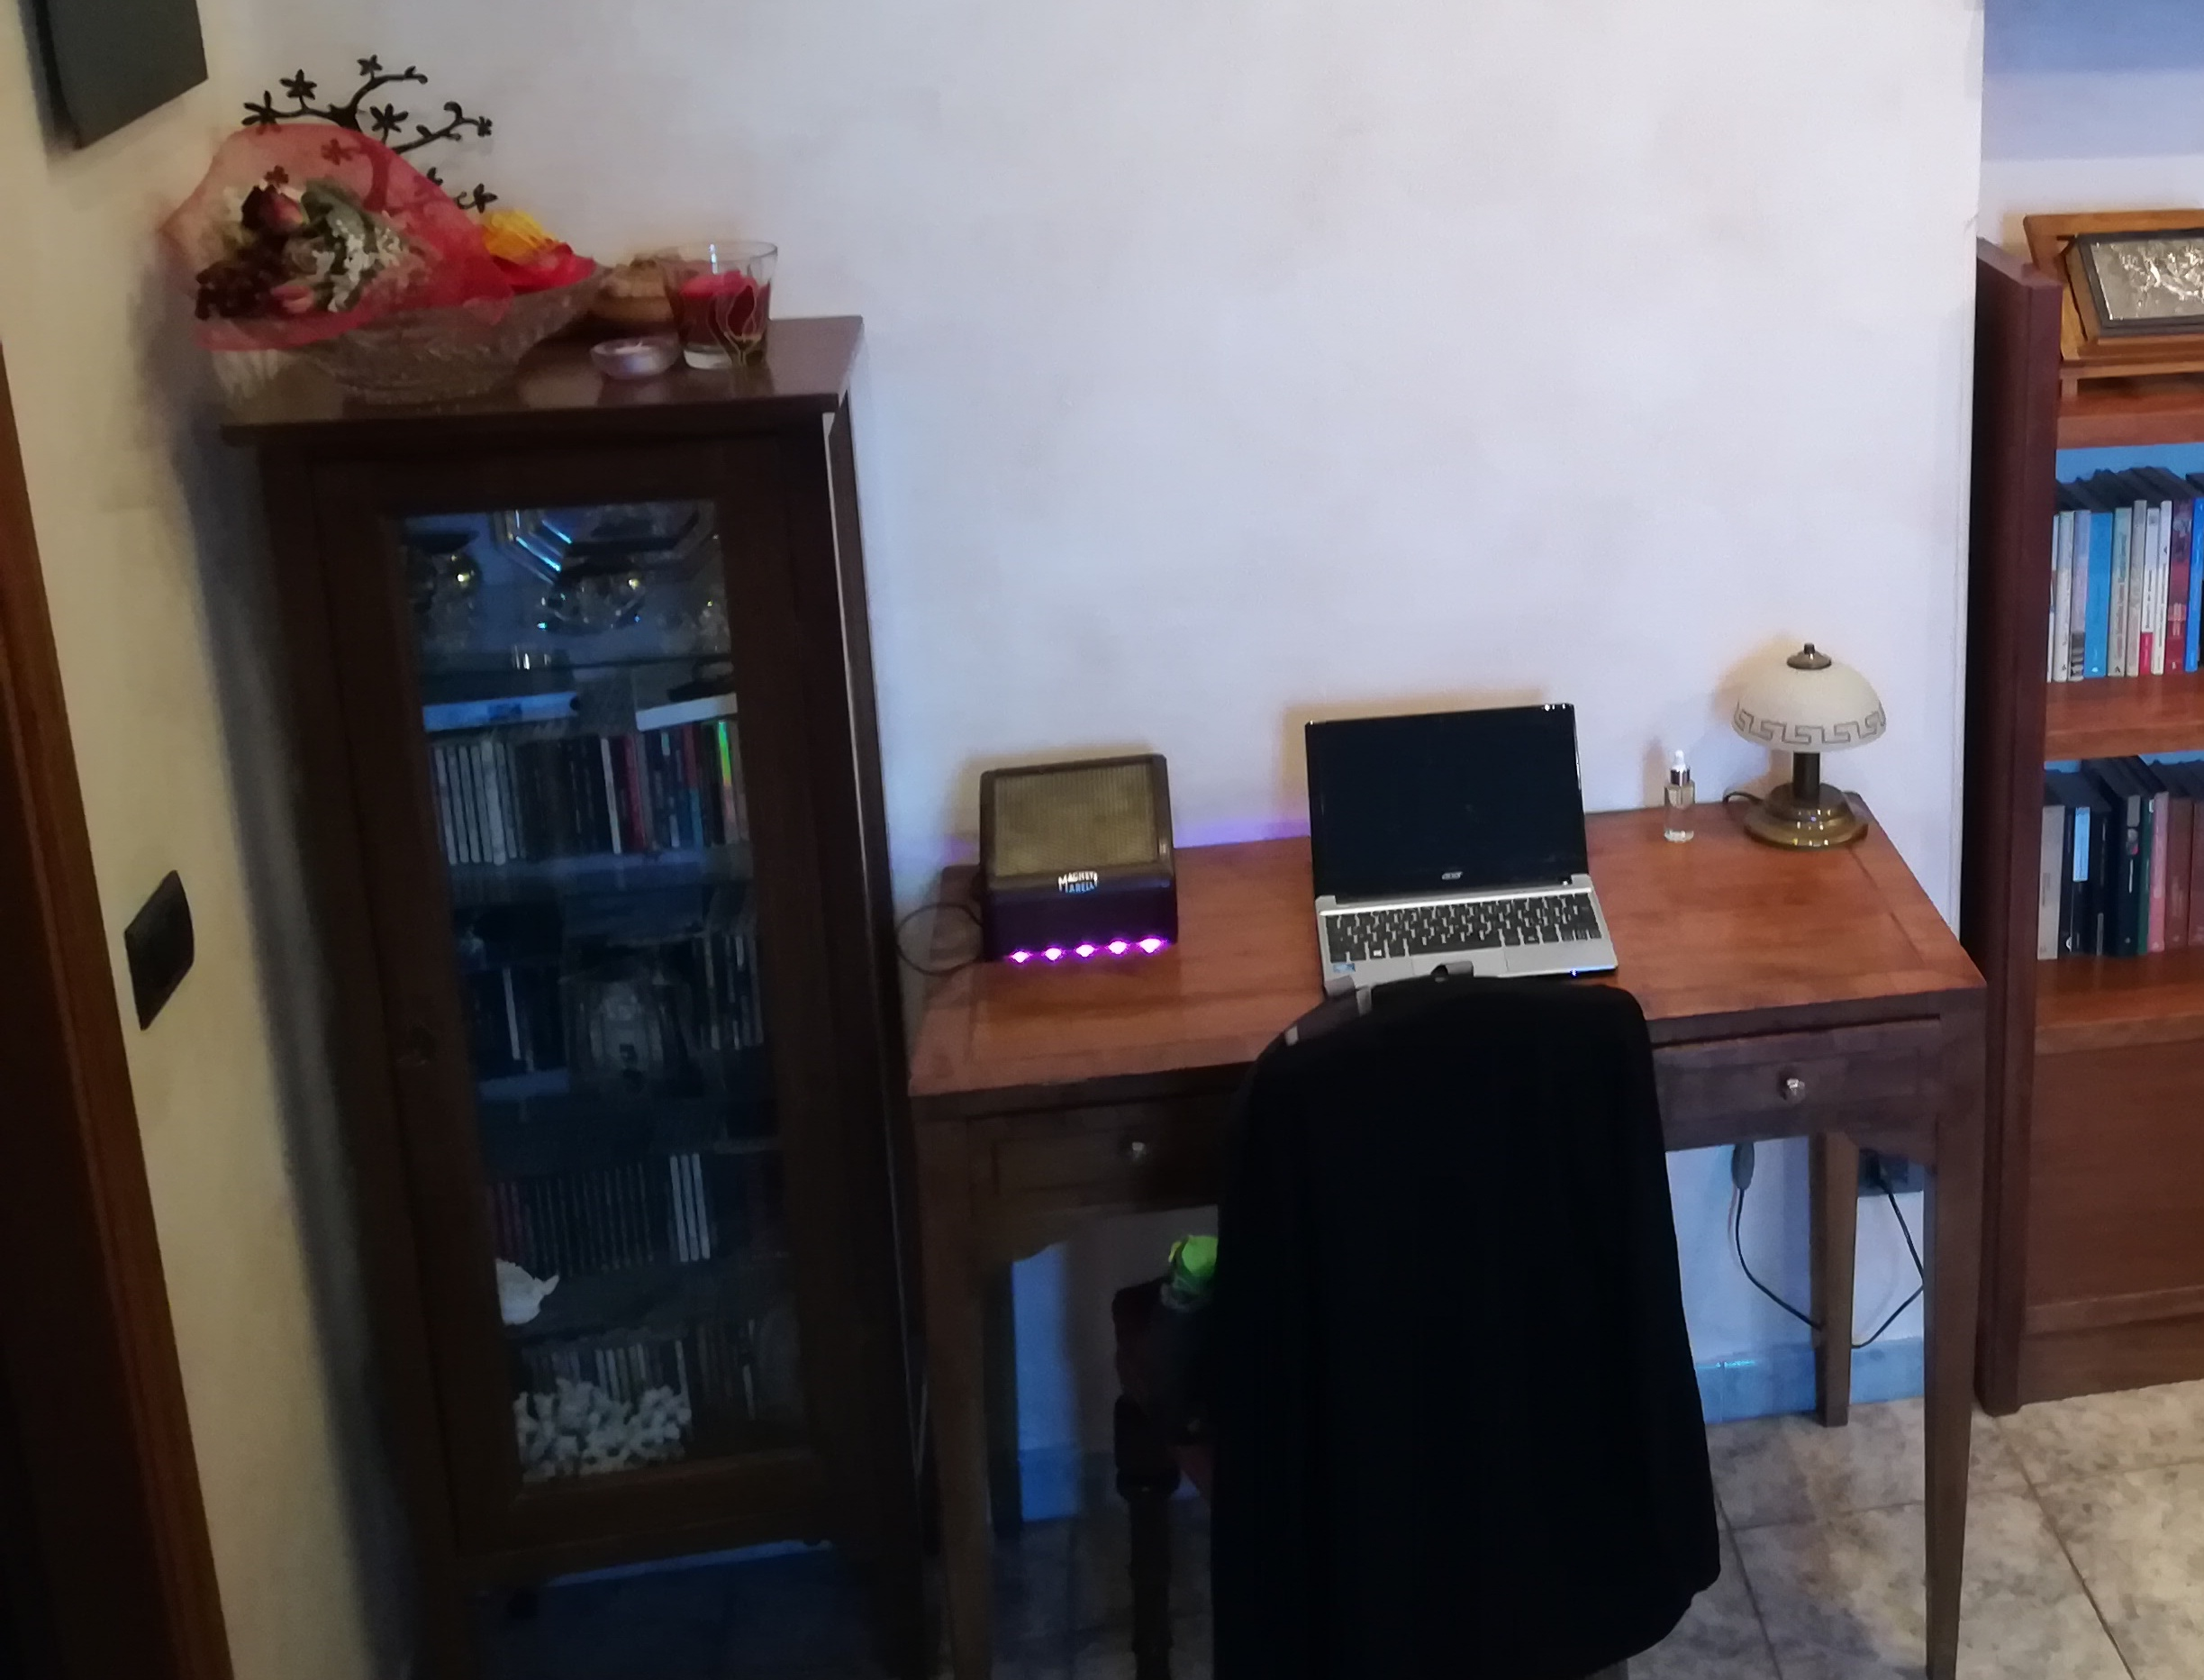
\includegraphics[width=.99\textwidth]{Immagini/Foto_Physiradio/blended/13.jpg}}
		\caption{\physiradio\ ``\textit{blended}" nell'ambiente, come un comune device IoT pensato per una smart home (suggerimento: cercare i led)}
		\label{fig:blended}
	\end{center}
\end{figure}

%In base alla definizione appena fornita, ci si è focalizzati su quelle tipologie di dispositivi, di piccole/medie dimensioni, direttamente collegati a una rete. 
%di solito hanno la capacità di trasferire i dati avanti e indietro senza intervento umano, possono essere semplici sensori / attuatori o dispositivi più complessi come assistenti personali per gestire le condizioni ambientali (ad esempio, aria condizionata, cucina, linee di produzione, ecc.).
%
%Per implementare un dispositivo che deve essere accettato da persone non tecniche, i creatori \physiradio\ hanno deciso di costruire un paio di apparecchi IoT all'interno di scatole di altoparlanti Magneti Marelli in legno vintage.


\chapter{Physiradio: ideazione e realizzazione del device} 

Una volta capiti quali erano i dati da voler fisicalizzare, con quali criteri e come rappresentare la fisicalizzazione, si è giunti al momento di creare il prototipo. Il device è osservabile nel dettaglio alla Figura \ref{fig:physiradio}
\bigskip
\begin{figure}[H]
	\begin{center}
		\centerline
		{
			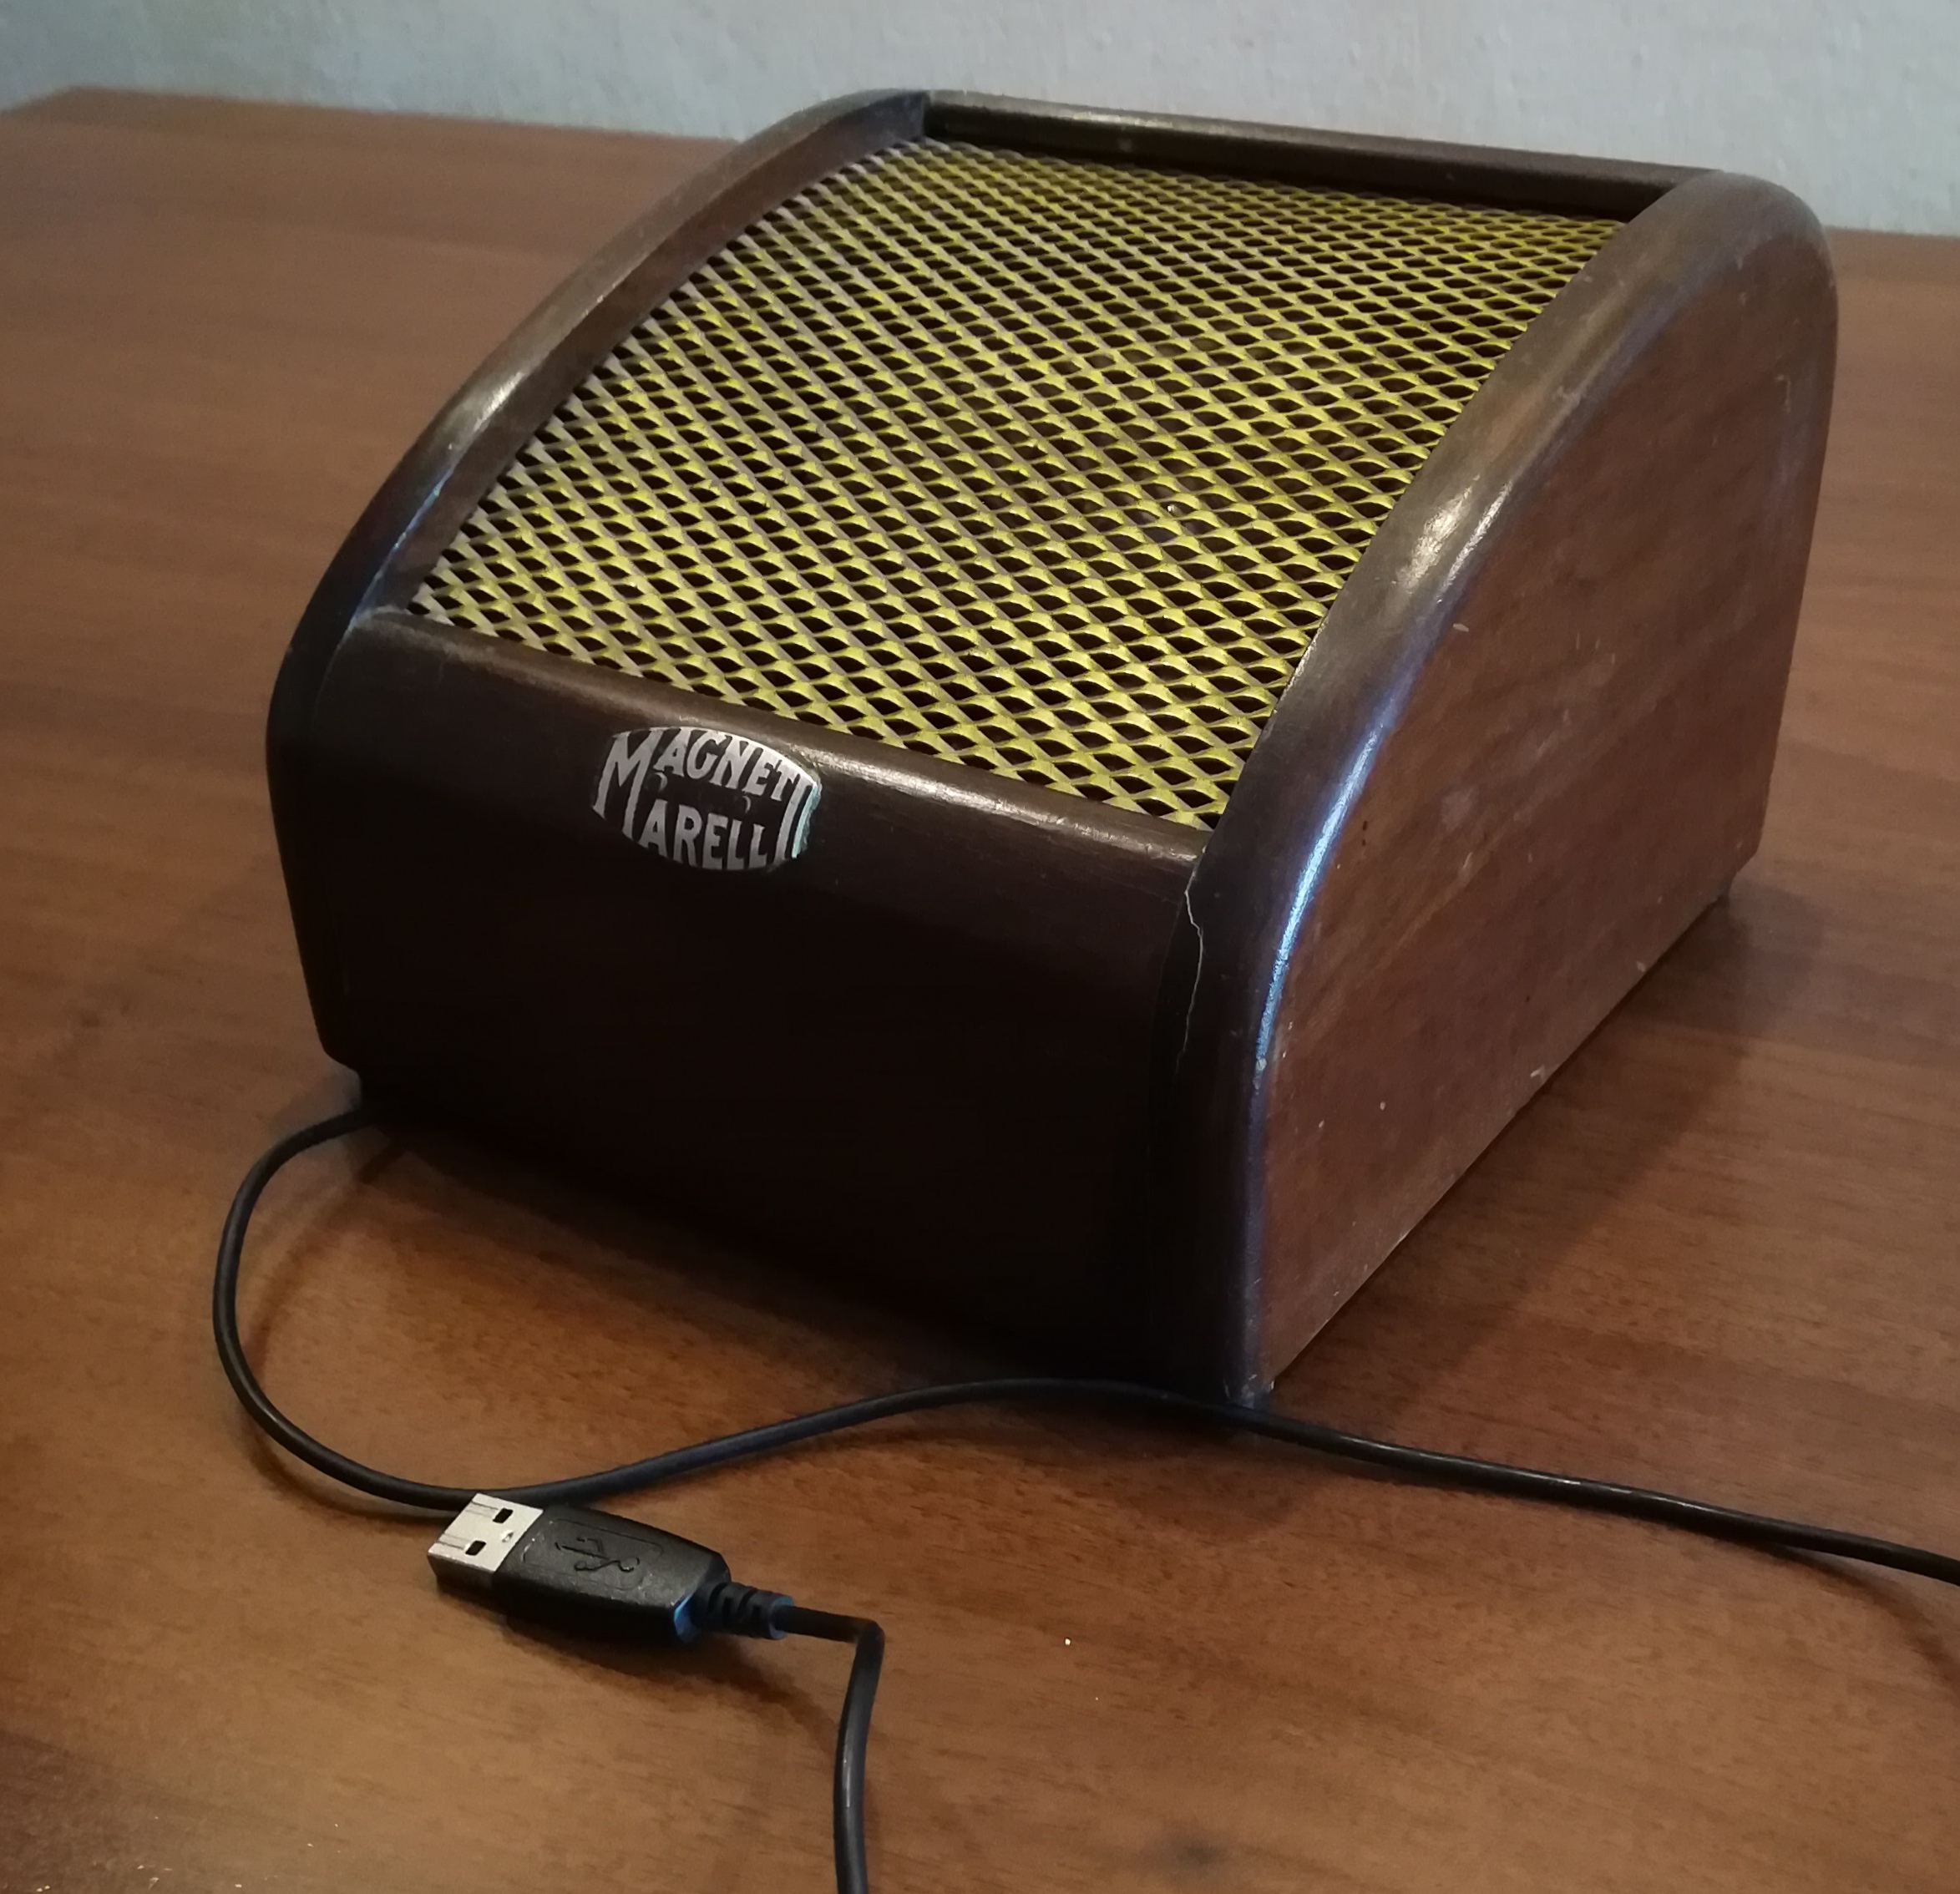
\includegraphics[width=.500\textwidth]{Immagini/Foto_Physiradio/old/MagnetiMarelli_1.jpg}
			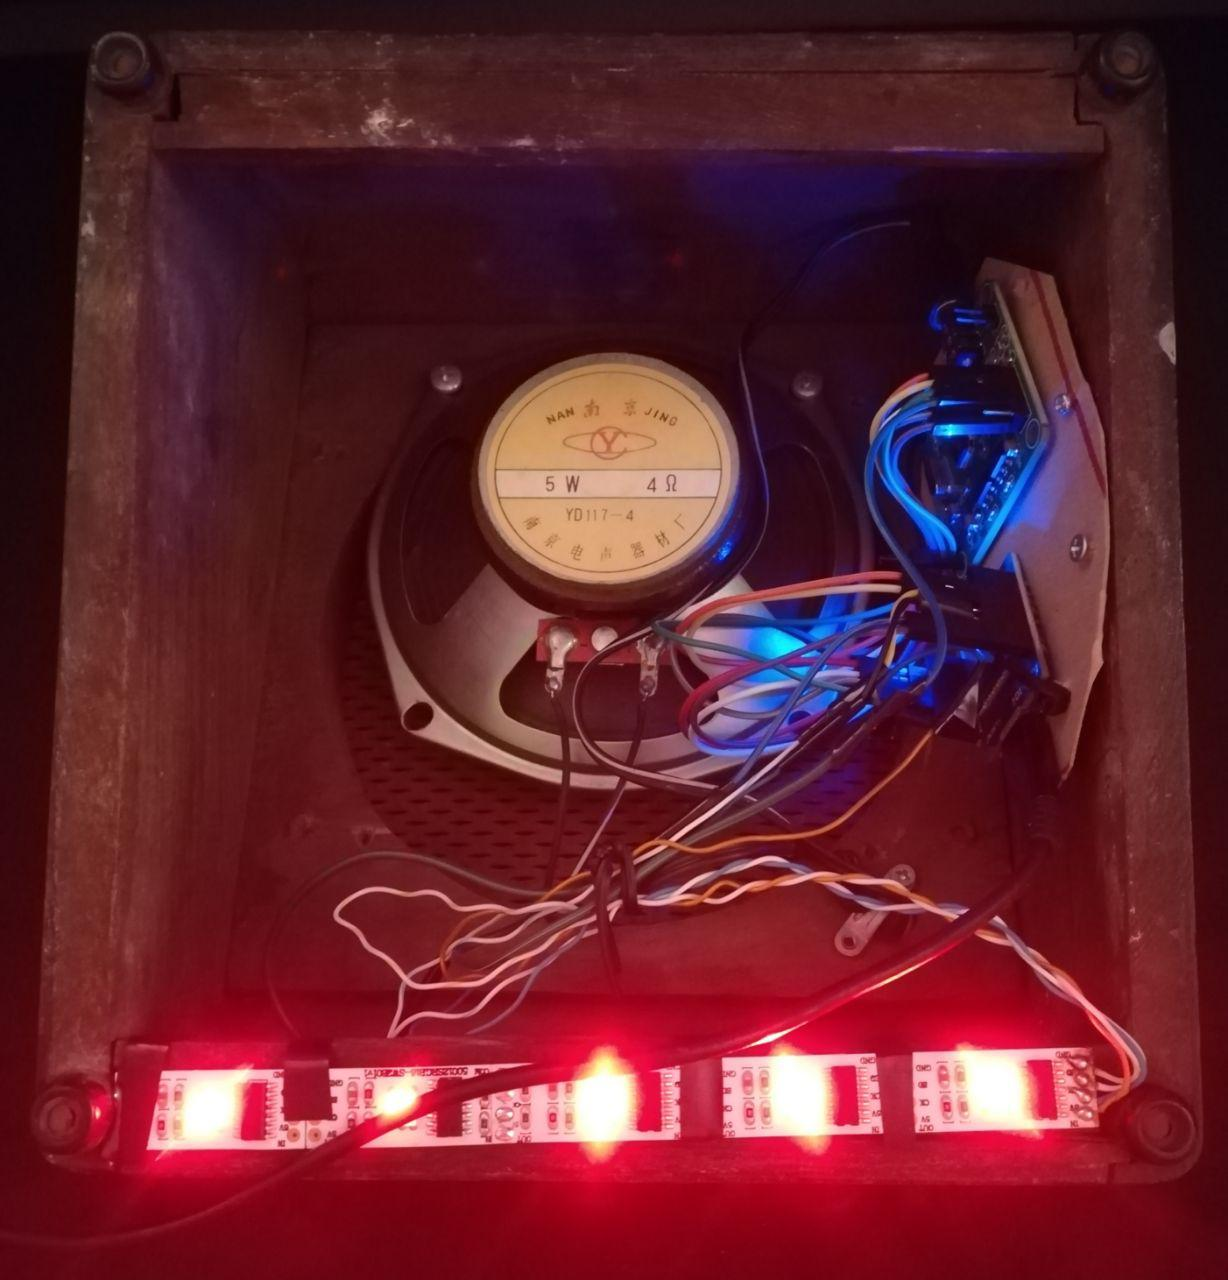
\includegraphics[width=.463\textwidth]{Immagini/Foto_Physiradio/old/MagnetiMarelliLed_2.jpg}
		}
		\caption{Il prototipo \physiradio\ visto: all'esterno (sinistra) e all'interno (destra)}
		\label{fig:physiradio}
	\end{center}
\end{figure}

Esso è composto dalle seguenti componenti: 
\begin{compactitem}
	\item Un cabinato vintage Magneti Marelli (anni '40 ca), con un piccolo speaker montato all'interno
	\item Una scheda embedded Wemos D1 Mini
	\item Un codec audio VS1053
	\item Una striscia led WS2801
\end{compactitem}

Nelle prossime sezioni verranno descritti nel dettaglio i componenti hardware utilizzati, come interagiscono tra di loro, e come i software implementati permettano le interazioni tra le varie parti. 

\section{Componenti Hardware}

Il fulcro di \physiradio\ è la board, una Wemos D1 mini. Ad essa sono connessi tutti gli altri componenti (eccezion fatta per lo speaker). %tramite cavi. 
Il funzionamento di tutto il dispositivo segue questa logica: il software che gira sulla scheda embedded riceve i dati riguardanti il tempo atmosferico, li interpreta e, successivamente, vengono \textit{in parallelo}: settati i led, per poter emanare uno specifico colore, e bufferizzati i byte relativi ai flussi audio, per poi essere mandati al codec audio, che li concretizza in segnale audio emettendo musica dallo speaker.
%Di seguito vengono analizzati nello specifico tutti i componenti hardware impiegati nel device. 

\subsection{Scheda embedded}\label{sec:wemos} %Wemos D1 mini

``Con la terminologia Sistema Embedded (tradotto testualmente ``sistema incorporato'') si tende ad indicare l’insieme composto da hardware e software (occasionalmente definito firmware) dedicato a specifici scopi (``\textit{specific purpose}'') i cui elementi siano tutti quanti integrati ed incorporati.'' \cite{sistemiembedded}

Per la creazione del device, si è optato, sin dalle prime fasi, di scegliere una scheda embedded piccola di dimensioni, ma che avesse abbastanza potenza di calcolo e feature che potessero garantire tutte le funzionalità necessarie al corretto funzionamento di \physiradio.
Di conseguenza, sia per scelte legate al budget, che per le appena citate motivazioni progettuali, la scelta è caduta su un Wemos D1 mini (Figura \ref{fig:wemosD1mini}).

\begin{figure}[h]
	\begin{center}
		\centerline{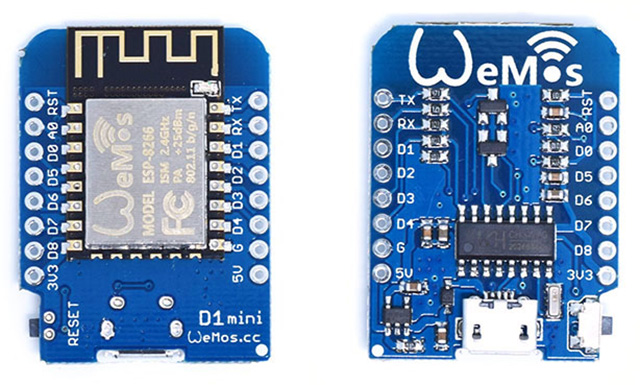
\includegraphics[scale=0.35]{Immagini/Wemos_Lolin_D1_mini_v1.jpg}}
		\caption{Scheda Embedded WeMos D1 mini (V1.0.0), fonte \cite{micheleMaffucciWemosV1}}
		\label{fig:wemosD1mini}
	\end{center}
\end{figure}

Essa è una piccola board, sia per peso che per dimensioni (34.2x25.6mm , 3g ca), creata da Wemos.cc \cite{wemosd1_mini}. 
È basato sul chip ESP-8266EX, dotato di un microprocessore Tensilica L106 a 32 bit, che presenta un consumo di energia estremamente basso, la cui velocità di clock della CPU può variare tra gli 80 e i 160 MHz.
Una grande dote del Wemos D1 mini, è il modulo ESP-12F: un modulo Wi-Fi 2.4 GHz IEEE 802.11 b/g/n, con supporto WPA/WPA2, che permette la realizzazione di numerosi progetti nell'ambito dell'IoT tramite l'accesso a reti locali.
Dispone inoltre di: 11 pin I/O digitali che gestiscono interrupt, pwm, I2C e ISP (tutti funzionanti con una tensione di alimentazione di 3,3 Volt), 1 ingresso analogico, una memoria flash interna di 4MB e un connettore mini USB, da cui viene anche prelevata un'alimentazione di 5 Volt (fondamentale per il funzionamento del codec audio).\\
Grazie a queste sue caratteristiche, sommate ad un basso prezzo di acquisto, la sua facile accessibilità e alla sua possibile programmazione attraverso l'IDE Arduino\cite{arduino}, questa board è divenuta molto popolare negli ultimi anni tra i ``maker'', sia hobbysti che professionisti.\\
Per implementare \physiradio\ è risultata la candidata ideale.
Si ringrazia Michele Maffucci \cite{micheleMaffucciWemosV1} per i credit dell'immagine e per le specifiche della versione V1.0.0, poiché attualmente la scheda è alla versione v.3.1.0 e sul sito ufficiale vi sono solo le specifiche dell'ultima versione. 


\subsection{Decodificatore audio}\label{sec:vs1053} %VS1053 Codec Audio

Per poter implementare il concetto di \textit{musicalization}, e di conseguenza riprodurre flussi audio per poter ascoltare le varie stazioni webradio, ovviamente è necessario un dispositivo che permetta di decodificare le informazioni ricevute dalla rete (dal Wemos D1 mini) e che, una volta bufferizzate, vengano riprodotte da una sorgente sonora. 
Per questo motivo, è risultato fondamentale l'utilizzo di un decodificatore audio, che potesse essere di dimensioni contenute e di basso costo, ma che potesse svolgere adeguatamente il lavoro.\\
La scelta perciò si è riversata su un VS1003/1053, in particolare il modello costruito dalla LC Technology, Figura \ref{fig:vs1053} .

\begin{figure}[h]
	\begin{center}
		\centerline{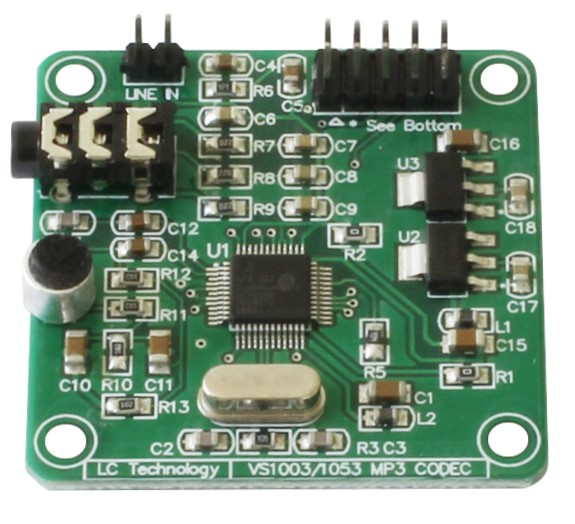
\includegraphics[scale=0.35]{Immagini/LCTech_VS1053.jpg}}
		\caption{LC Technology VS1003/1053 MP3 Codec audio, fonte \cite{lcTechnologyVS1053}}
		\label{fig:vs1053}
	\end{center}
\end{figure}

Il modulo di codec audio VS1053 è sia un decodificatore audio MP3/MP3 + V/WMA/WAV/MIDI/SP-MIDI completo, che un codificatore ADPCM, di piccole dimensioni (50x40.5 mm)  il quale presenta un DAC stereo (convertitore da digitale ad analogico), un ADC regolabile da 16 bit (convertitore da analogico a digitale), un driver cuffie stereo (con uscita jack da 3.5mm) , e tante altre feature importanti, consultabili direttamente sul sito del produttore \cite{lcTechnologyVS1053}.\\
Delle caratteristiche di questa scheda, ci soffermeremo solo su quelle fondamentali per il funzionamento di \physiradio.

L'alimentazione è di 5 Volt, a corrente continua, ed è erogata dal Wemos D1 mini (pin 5v). 
%Il driver cuffie ha un'impedenza di 30 Ohm, che è un valore molto basso\todo{atrent: rispetto a cosa? gli speaker sono in genere d 8 Ohm quindi 30 è alto ;) simo: io sapevo che quando si parla di driver cuffie tendenzialmente fino ai 32ohm si parla di bassa impedenza}, il che permette di emettere suoni, dalla fonte collegata all'output jack, senza aver bisogno di tanta potenza. Di fatti il rapporto tra tensione (5Vdc) e l'intensità di corrente massima erogata di 800mAh, garantisce una potenza di max 4 Watt \todo{atrent: magari! avresti un'efficienza del 100\%}, che ad esempio per un piccolo altoparlante, è più che sufficiente.\\
Utilizzando il driver per cuffie, si può alimentare in maniera congrua lo speaker, ottenendo un sufficiente volume d'ascolto.\\ %\todo{simo to atrent: ho collassato le frasi in questa}
Inoltre il modulo è munito di un'interfaccia SPI (Serial Peripheral Interface), ovvero un sistema di comunicazione seriale tra un microcontrollore e altri circuiti integrati, o tra più microcontrollori, fondamentale per il prototipo. \\
Nello specifico, la board Wemos funge da master e il VS1053 da slave, in modo tale che dalla board venga emesso il segnale di clock per sincronizzare la comunicazione. Conseguentemente, il traffico viene gestito tramite un buffer di 32 byte (poiché è la capienza massima gestibile dal codec audio) presente in entrambe le schede. Viene riempito prima il buffer del Wemos D1 mini con lo stream acquisito dalla rete, trasferito al buffer del decodificatore audio, che lo interpreta, trasformandolo in un segnale analogico, ossia la musica.\\
Quest'ultimo passaggio è reso possibile grazie alla libreria creata da Marcin Szałomski \cite{vs1053baldram}, senza la quale sarebbe stato molto complesso ottenere una comunicazione tra le due componenti.

\subsection{Speaker e striscia led}
Le ultime componenti hardware da descrivere sono già state introdotte con la presentazione del prototipo (Figura \ref{fig:physiradio}), ovvero lo speaker e la striscia led.
Per quanto riguarda la prima, è uno speaker realmente vintage della Magneti Marelli. Si specifica tuttavia che solamente il cabinet in legno è originale, risalente circa agli anni '40, poiché lo speaker vero e proprio è moderno, di dimensioni ridotte; con impedenza 4 Ohm e potenza massima iniettabile di 5 W, il che lo rende adatto alle caratteristiche del decodificatore audio descritto nella sezione precedente.\\

La striscia led invece, è una WS2801, ovvero una led strip digitale a quattro pin: alimentazione (5V), ground (GND), clock (CLK) e data (SD). 
Per adattarsi comodamente al cabinet in legno, con un \textit{cable management} semplice, sono stati utilizzati solamente cinque led, posizionati nella parte frontale della struttura (sotto il logo `Magneti Marelli') che puntano verso il basso. Questo garantisce una visione sufficiente del colore.
%\todo{atrent: perché? spiegalo. simo: va bene cosí? atrent:ok}

Una nota da specificare è relativa al fatto che, sebbene sia digitale, quindi che ogni led è controllabile singolarmente via codice (trattandolo come un vero e proprio array), per questa prima versione del prototipo la \textit{led strip} è utilizzata come se fosse una striscia led analogica, senza quindi animazioni o controlli particolari dei led. 


\subsection{Schema cablaggio} 

Nella Figura \ref{fig:schemaFritzing}, viene riportato un semplice schema elettronico per dare un'idea di quali siano i collegamenti tra le quattro componenti hardware utilizzate per la creazione del prototipo, che sono state esplicitate in modo più chiaro sulla tabella \ref{tab:wirings}. Lo schema è stato realizzato con Fritzing \cite{fritzing}, un software libero pensato per la Electronic Design Automation (EDA), ovvero la progettazione di componenti elettroniche. \\


\begin{center}
	\begin{figure}[H]
		\begin{center}
			\centerline{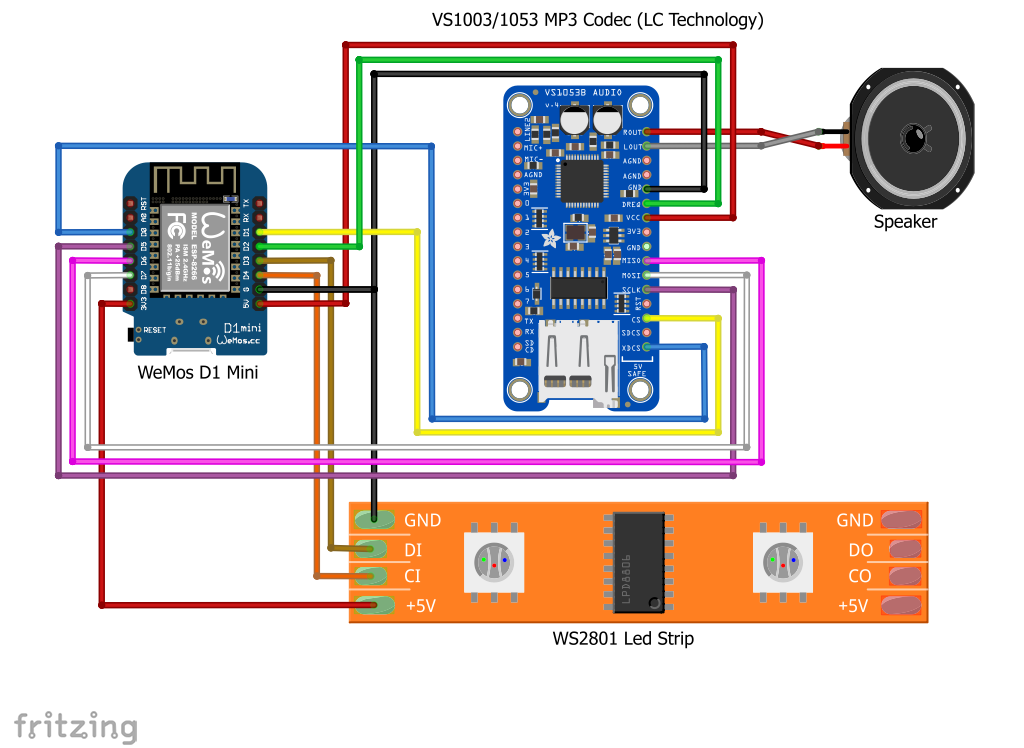
\includegraphics[scale=0.6]{Immagini/SchemaWiringsFritzing.png}}
			\caption{Schema Fritzing del cablaggio delle varie componenti hardware all'interno di Physiradio}
			\label{fig:schemaFritzing}
		\end{center}
	\end{figure}
	
	\begin{table}
		\centering
		\begin{tabular}{|c|c|c|c|}
			\hline
			\textbf{Wemos D1 mini} & \textbf{VS1053} & \textbf{WS2801} \\
			\hline
			D0 & DCS & - \\  
			\hline
			D1 & CS & - \\
			\hline
			D2 & DREQ & - \\
			\hline
			D3 & - & SD \\
			\hline
			D4 & - & CLK  \\
			\hline
			D5 & SCK & -  \\
			\hline
			D6 & MISO & -  \\
			\hline
			D7 & MOSI & -  \\
			\hline
			5V & +5V & -  \\
			\hline
			3V3 & - & +5V  \\
			\hline
			G & GND & GND  \\
			\hline	
		\end{tabular}
		\caption{Schema cablaggi interni a \physiradio\ }
		\label{tab:wirings}	
	\end{table}
\end{center}

Occorre però specificare alcuni dettagli implementativi, in quanto si è dovuto ricorrere ad un \textit{cable management} ottimale per poter far funzionare correttamente tutte le componenti e farle coesistere all'interno della struttura di \physiradio\ : 
\begin{compactitem}
	\item È stato necessario saldare appositamente un cavo per poter avere il ground sia per il codec audio che per la striscia led, visto che il Wemos D1 mini possiede un solo pin per il ground (vedere Figura \ref{fig:wemosD1mini});
	\item Come si può notare nella tabella \ref{tab:wirings}, si è deciso di alimentare la striscia led con una tensione di 3.3 Volt e non 5 Volt come suggerito, semplicemente per comodità pratica; visto e considerato che anche un'alimentazione più scarsa è sufficiente per generare luce da dei led;
	\item Il canale sinistro e il canale destro dello speaker, sono saldati ad un jack 3.5mm che è inserito direttamente nell'ingresso jack del VS1053, poiché è sufficiente l'amplificatore interno al codec audio per produrre del suono ad un volume accettabile. 
\end{compactitem}

\medskip
Inoltre vanno specificati alcuni dettagli riguardanti lo schema. Il modulo audio non è lo stesso usato nel dispositivo reale: Il codec nello schema è un Adafruit VS1053, poiché purtroppo il modello della LC Technology (Figura \ref{fig:vs1053}) non esiste per Fritzing, e questo è il più simile trovato in rete. Lo stesso discorso vale per la striscia led, dove nella WS2801, utilizzata nel dispositivo, il pin CI è CLK (clock) e DI è SD (data).

\newpage
\section{Software implementati e utilizzati}

Dovendo programmare una board come il Wemos D1 mini, la maggior parte dello sviluppo del codice si è incentrata su uno script per Arduino IDE \cite{arduino}, un'applicazione multipiattaforma open source, che offre all'utente un editor di testo per permettere la stesura di codice sorgente. Oltre al supporto di tutte le board Arduino, permette l'installazione di librerie atte a supportare gran parte dei sistemi in commercio, come il NodeMCU ESP8266, l'ESP32, i Wemos e molti altri, la cui scelta si basa sul tipo di utilizzo previsto.\\
In questi paragrafi verranno trattati quali protocolli e quali librerie sono stati utilizzati per il funzionamento del prototipo. Nello specifico verrà trattato il protocollo MQTT, la libreria multitasking e le funzionalità introdotte per interagire col device.\\
È utile precisare che, all'interno dello script, viene utilizzata la libreria ArduinoJSON \cite{arduinoJSON}, che è stata fondamentale al fine di poter interpretare i file di tipo JSON, ricevuti tramite le API di OpenWeatherMap, per poter ottenere le condizioni atmosferiche della città interrogata.\\
%\todo{simo to atrent: ho parlato di rado del JSON, dimmi tu se ha senso inserirlo oppure no. atrent: una frase ci sta, visto che cmq hai fatto excursus su ogni aspetto del device. simo: messo qui - atrent:ok}


In un secondo momento è stata sviluppata un'applicazione su Unity\cite{unity} per dare un esempio di come si può interagire con \physiradio\ in contesti più realistici, rispetto allo stato attuale del device che è comunque prototipale.

%\subsection{Arduino IDE}
%\todo{simo to atrent: ho collassato la sezione nell'intro dei software}



\subsection{Il protocollo MQTT} \label{sec:mqttProtocol}

MQTT \cite{mqttOfficial} è l'acronimo di Message Queue Telemetry Transport; le cui versioni v3.1.1 e v5.0 sono standard OASIS dal 2014 (la v3.1.1 è stata anche ratificata dalla ISO). \\
È un protocollo di messaggistica di pubblicazione/sottoscrizione (\textit{publish/subscribe}), estremamente semplice e leggero, progettato per dispositivi con risorse limitate e/o poco prestanti, e per reti a bassa larghezza di banda, alta latenza o inaffidabili. \\
I principi di progettazione sono quelli di minimizzare sia la banda utilizzata della rete che i requisiti delle risorse del dispositivo, cercando allo stesso tempo di garantire affidabilità e un certo grado di garanzia della consegna dei messaggi. Questi principi, si sono rivelati col tempo ideali per rendere il protocollo molto utile e sfruttato dal mondo emergente dei dispositivi interconnessi ``\textit{Machine-to-Machine}'' (M2M) e del ``\textit{Internet of Things}'' (IoT), e per le applicazioni mobile, in cui la larghezza di banda e la durata della batteria sono fondamentali.

Prendendo come descrizione di riferimento \cite{sistemiembedded}: Il protocollo si appoggia principalmente al protocollo TCP/IP, o in alternativa ad altri protocolli di rete che forniscono connessioni ordinate, senza perdita di dati e bidirezionali. Esso si basa sul pattern \textit{publish-subscribe}\footnote{Inteso come Design Pattern, sul modello  Observer-Observable}: dei messaggi informativi vengono inviati da una sorgente (un nodo ``client'' della rete MQTT) verso un \textit{dispatching broker} che li ridistribuisce a tutti i nodi che si erano dichiarati interessati a quel tipo (topic) di messaggio.\\
Ogni messaggio MQTT è composto da:

\begin{compactitem}
	\item un \textit{topic}, che servirà al broker per la distribuzione: è una stringa il cui contenuto è libero, ma viene specificata la forma sintattica da utilizzare per costruirlo (parole separate dal carattere ``/'', vedere documento di markdown nella sezione \ref{sec:descriptionInteraction} per degli esempi);
	\item un \textit{payload}, il corpo del messaggio: è semplicemente una stringa UTF-8, la cui semantica è affidata alle convenzioni stabilite tra chi manda e chi riceve, non è definita nel protocollo.
\end{compactitem}

Il broker gestisce una lista di nodi client interessati ai vari topic, ogni messaggio che riceve viene inviato solo ai nodi che si erano “iscritti” a quel particolare topic. I nodi che si ``iscrivono"(\textit{subscribe}) possono indicare come “interesse” anche una \textit{wildcard}, una stringa contenente caratteri speciali che rappresenta un insieme di stringhe effettive (si veda la funzione \texttt{reconnect()} nel \nameref{Codice 1.1}, Appendice A, per avere un esempio), invece di un singolo topic per esteso.\\
È perciò un modello che fornisce la distribuzione dei messaggi uno-a-molti e il disaccoppiamento delle applicazioni.\\

Un'altra caratteristica specifica del protocollo MQTT, sono i livelli di Quality of Service (QoS), letteralmente qualità di servizio. 
È un accordo tra il mittente e il destinatario del messaggio, che ne definisce la garanzia di consegna.
I livelli QoS sono una funzionalità chiave del protocollo MQTT, perché offre al client la possibilità di scegliere un livello di servizio che corrisponda all'affidabilità della rete e alla logica dell'applicazione. Poiché MQTT gestisce la ritrasmissione dei messaggi e garantisce la consegna (anche quando il trasporto sottostante non è affidabile), i livelli QoS rendono molto più semplice la comunicazione con reti inaffidabili.\\
I QoS sono 3 livelli, e sono: 
\begin{itemize}
	\item \textit{``At most once"} - QoS 0, in cui i messaggi vengono recapitati in base ai migliori sforzi dell'ambiente operativo. La perdita del messaggio può verificarsi, ma è il metodo più veloce per inviarlo. 
	
	\item \textit{``At least once"} - QoS 1, in cui è garantito l'arrivo dei messaggi tramite un ACK specifico (PUBACK) inviato dal broker. Possono verificarsi duplicati.
	
	\item \textit{``Exactly once"} - QoS 2, dove è garantito che il messaggio arrivi esattamente una volta, tramite un four-part handshake tra client e broker. È ovviamente il metodo più lento, ma anche il più sicuro.
\end{itemize}

Tutti i messaggi inviati con QoS 1 e 2 vengono messi in coda per i client offline, fino a quando il client non sarà nuovamente disponibile. Tuttavia, questo è possibile solo se il client ha una sessione persistente.\\
%Riduzione del traffico di rete e scambi di protocollo ridotti al minimo per ridurre il traffico di rete.
% Un meccanismo per informare le parti interessate quando si verifica una disconnessione anomala.\\

\medskip

È necessario specificare che, in tutti i software sviluppati per questo progetto, si è sempre utilizzato il livello Quality of Service 0. 
La ragione principale di questa scelta, è legata al fatto che le componenti utilizzate per creare il device hanno risorse molto limitate e poco prestanti, specialmente la scheda embedded, che è di fatto il nucleo del funzionamento del prototipo. Di conseguenza, con un QoS 0, possiamo comunque ottenere un sistema rapido ed efficiente per quello che è il suo scopo; senza però avere meccanismi di sicurezza e di check del messaggio inviato. Viene dunque tenuto in considerazione, che un messaggio potrebbe non essere recapitato a \physiradio, il che non è problema considerando il tipo di dato che viene trasferito sulla rete: privo di dati sensibili e che se, anche sniffato e/o alterato, non causerebbe rischi eccessivi a livello di sicurezza. \\

\medskip 

Nelle varie implementazioni di MQTT (è disponibile per molti linguaggi, sistemi operativi e su piattaforme sia embedded che standard) le funzioni principali le due:
%\todo{atrent: qui puoi usare texttt per i pezzi piccoli di codice e funzioni. simo: ok grazie}


\begin{compactitem}
\item \texttt{Subscribe(String subTopic, Function callback)}: permette (una volta connessi ad un broker) la dichiarazione di interesse verso uno o più topic, quando il broker riceve un messaggio il cui topic corrisponde con subTopic lo invia al client che lo riceve e scatena l’invocazione della funzione callback che va implementata a cura del programmatore del nodo “\textit{subscriber}”;
\item \texttt{Publish(String topic, String message)}: permette (una volta connessi ad un broker) l’invio di un messaggio associato ad un topic, il broker analizzerà il topic e inoltrerà il messaggio ai nodi il cui subTopic corrisponde.
\end{compactitem}

\medskip

In questo progetto, il protocollo è stato implementato grazie alla libreria (per Arduino IDE) PubSubClient \cite{mqttPubSubClient}, creata da Nick O’Leary. Il codice implementato (\nameref{Codice 1.1}) è visionabile all'Appendice A. Nello specifico si può notare che sono state utilizzate le seguenti funzioni:
\begin{compactitem}
	\item \texttt{setServer (server, port)} : indirizzo e porta del server a cui connettersi;
	\item \texttt{setCallback (callback)} : un puntatore a una funzione di callback del messaggio, chiamata quando arriva un messaggio per la sottoscrizione a uno(o più) topic creato dal client. La funzione di callback ha questa forma: \\
	
	\texttt{void callback(const char[] topic, byte* payload, unsigned int length)}\\
	
	e i parametri sono:\\
	\texttt{topic const char[]} - il topic sul quale è arrivato il messaggio;\\
	\texttt{payload byte[]}- il payload del messaggio;\\
	\texttt{length unsigned int} - la lunghezza del payload.\\
	
	\item \texttt{subscribe (topic, [qos])} : sottoscrive il client ai messaggi pubblicati dal server su uno specifico topic. Si può decidere opzionalmente con quale livello di QoS sottoscriversi al server;
	\item \texttt{connected ()}: verifica se il client è connesso ad un server;
	\item \texttt{connect (clientID, [username, password], [willTopic, willQoS, willRetain, willMessage], [cleanSession])}: cerca di connettersi al server settato precedentemente (con la funzione setServer). Si può opzionalmente conferire username e password, se il server li richiede per istanziare la connessione. Inoltre si possono settare i parametri legati al Last Will and Testament (LWT), per informare gli altri \textit{subscriber} dello stesso broker che il client si è disconnesso (di solito in modo anomalo). Per ultimo, si può settare opzionalmente se il client richiede una connessione persistente(non-clean) oppure no.\\
\end{compactitem}
Occorre specificare che non è mai stata usata alcuna funzione di \textit{publish}, poiché \physiradio, allo stato attuale di sviluppo, è pensato solo per ricevere, analizzare e interpretare i messaggi che vengono inviati dai client \textit{publisher}. 

\subsection{Libreria TaskScheduler}

Un altro punto fondamentale del funzionamento di \physiradio\ è la sua implementazione del \textit{multitasking}.
%Quando si parla di sistemi embedded, i cui software sono stati sviluppati su Arduino IDE, parliamo di sistemi monoprogrammati, in quanto non sono previsti meccanismi di \textit{time sharing} (per il programma scritto dall'utente). 
%Questo approccio di sviluppo tuttavia è limitante, spesso comporta la gestione di un numero limitato di funzionalità; e se si vogliono gestire molteplici \textit{task}, spesso si ricorre a tecniche naïf, con poche, se non nulle, politiche di scheduling.\\
%Tuttavia, durante le prime fasi di sviluppo del device, è subito sorto il problema di dover implementare un sistema \textit{multitasking}, che gestisse le tre principali funzionalità del software: 

Quando si parla di sistemi embedded, i cui software sono stati sviluppati su Arduino IDE, vi sono numerose librerie per gestire, in modo elegante, più flussi paralleli all'interno del programma utente; nella logica di pulizia del codice, senza di esse, spesso si ricorre a tecniche naïf \footnote{In gergo si parla di ``gestire a mano a colpi di millis'' i vari task}.\\
Durante le prime fasi di sviluppo del device, è subito sorto il problema di dover gestire le tre principali funzionalità del software: 

\begin{compactitem}
	\item Flusso continuo dello streaming audio, reindirizzato al codec audio;
	\item Interrogazione del sistema OpenWeatherMap, per avere il dato da mappare in \textit{real-time};
	\item Ricezione di messaggi MQTT che arrivano dal broker.
\end{compactitem}  
E che, di conseguenza, fossero gestite in modo ordinato e il più deterministico possibile, tramite delle politiche di scheduling. \\
A tal proposito, si è deciso di sfruttare una libreria per Arduino IDE, sviluppata da Anatoli Arkhipenko, chiamata TaskScheduler \cite{taskScheduler}.

\begin{figure}
	\begin{center}
		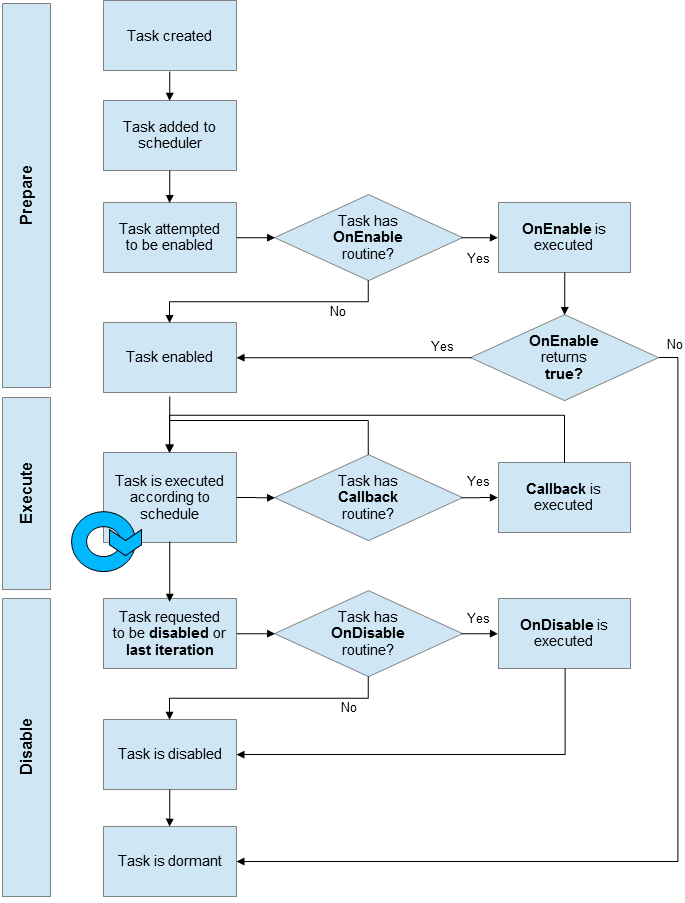
\includegraphics[width=0.85\textwidth]{Immagini/TaskScheduler_html.png}
		\caption{Workflow di TaskScheduler, fonte \cite{taskScheduler}}
		\label{fig:schemaTaskScheduler}
	\end{center}
\end{figure}

È un'implementazione, di dimensioni contenute, di un \textit{cooperative multitasking}, chiamato anche \textit{multitasking non-preemptive}.
Consiste sostanzialmente in una modalità di \textit{multitasking}, in cui il sistema operativo (nel nostro caso, con un ESP8266 compilato con le SDK Arduino, parliamo solamente di firmware \cite{wikiesp8266}) non avvia mai un \textit{context switch} da un processo in esecuzione ad un altro processo. Sono invece i processi stessi che volontariamente lasciano il controllo: periodicamente, o quando entrano in idle o quando vengono esplicitamente bloccati da qualche logica del programma. Questo tipo di \textit{multitasking} è chiamato ``cooperativo" perché tutti i processi devono cooperare per l'intero \textit{workflow} di scheduling (Figura \ref{fig:schemaTaskScheduler}) al fine di garantire l'esecuzione dell'intero programma.\\
Nel caso della libreria TaskScheduler, avremo un unico programma utente che gira all'interno della CPU, nel quale potremo creare dei processi (cosa che nativamente non è possibile fare su Arduino Ide), che per lo specifico si chiamano \textit{task}, e saranno tutti aggiunti ad una lista di task eseguibili all'interno di un oggetto Scheduler (vedere il \nameref{Codice 1.2}, Appendice B, per avere un esempio). Di default, i \textit{task}, vengono eseguiti ciclicamente a periodicità definite nel \textit{setup}, ma possono essere definiti molteplici parametri che ne possono variare notevolmente il ciclo di esecuzione.\\ 
In particolare, la libreria è in grado di garantire: l'esecuzione periodica dei \textit{task} espressi in millisecondi o microsecondi (se esplicitamente abilitato), il numero esatto delle iterazioni dei singoli \textit{task}, la modifica dinamica dei parametri di esecuzione (frequenza, numero di iterazioni, metodi di callback) e molte altre feature (vedere la documentazione ufficiale per info più specifiche \cite{taskScheduler}). 


%\todo{simo to atrent: spiegare nel dettaglio anche le funzioni? per ora spiego solo l'istanza atrent: no, fin troppo così}
Nel dettaglio, per l'implementazione di \physiradio\ è stata sfruttata principalmente la prima feature sopracitata, ovvero quella di definire l'esecuzione periodica dei singoli task, lasciando l'ordine di esecuzione con i parametri di default. È stata definita tramite un costruttore della classe Task:\\
\texttt{Task(unsigned long aInterval, long aIterations, void (*aCallback)(), \\
		Scheduler* aScheduler, bool aEnable,\\
		bool (*aOnEnable)(), void (*aOnDisable)());}\\
definendo \textit{aInterval}, l'intervallo di tempo ogni quanto eseguire il task, \textit{aInterations}, per quante volte eseguirlo, e assegnando \textit{*aCallback}, la funzione di callback da eseguire. Gli altri parametri, opzionali, non sono stati settati all'interno del costruttore, ma fuori da esso, per semplice comodità di debugging.\\
La sezione di codice sviluppata usufruendo della libreria TaskScheduler è visionabile all'Appendice B: da notare che, le tre principali funzionalità di \physiradio\ sopracitate, sono state tradotte in tre task specifici.\\  

%%%	CODICE TASK SCHEDULER 

\subsection{Descrizione dell'interazione con il device} \label{sec:descriptionInteraction}

Ci sono principalmente due modi per interagire con \physiradio: il primo metodo è quello di utilizzare l'app Physiradio MQTT Interface, che verrà descritta nel dettaglio successivamente (sezione \ref{sec:app}). Il secondo metodo consiste nell'utilizzare un qualsiasi device capace di eseguire il comando (del protocollo MQTT) \textit{publish}, interagendo con, o tramite, un broker MQTT. \\
In particolare, di seguito viene riportato integralmente  il documento di markdown (tradotto in italiano), disponibile sulla repository dedicata unicamente ai software di \physiradio\ \cite{repositorySwOnly}, dove vengono riportate le istruzioni, e degli esempi, per interagire con il device, nei quali viene utilizzato Mosquitto \cite{mosquitto} su un normale terminale Linux. \\ %\todo{atrent: ma è maschile o femminile? io lo davo per maschile. simo: su internet sono un po'divergenti i pensieri, tra colleghi noi abbiamo sempre detto LA repo, peró se pensi sia una cavolata lo cambio in tutto il testo}

\newpage
\hrule
\medskip

{\large\textbf{Topic e payload per interagire con PhysiRadio}}\\

\textbf{ATTENZIONE: Tutte le chiamate MQTT devono essere eseguite da un dispositivo capace di istanziare almeno un comando di MQTT \textit{publish} (per esempio un Mosquitto client o simili)}\\

Forma generica di istruzione: 

\begin{lstlisting}[style=customBash]
mosquitto_pub -h server_name -t PhysiRadio/topic -m "payload"
#nota: il "payload" deve essere scritto tra virgolette
\end{lstlisting}

\medskip 

{\large\textbf{Comandi eseguibili, divisi per topic:}}

\textbf{Volume}

\begin{compactitem}
	\item
	Volume +1
	\item
	Volume -1
	\item
	Volume mute
	\item
	Volume unmute
\end{compactitem}

Esempi:
\begin{lstlisting}[style=customBash]
mosquitto_pub -h server_name -t PhysiRadio/Volume -m "+1"
mosquitto_pub -h server_name -t PhysiRadio/Volume -m "mute"
\end{lstlisting}


\textbf{City (nota bene: la città deve esistere sulla piattaforma OpenWeatherMap, e il nome deve essere scritto possibilmente in lingua inglese)}

\begin{compactitem}
	\item
	City ``nome\_di\_una\_città" (non è case sensitive, grazie alle API di OpenWeatherMap)
	\item
	City ``nome\_di\_una\_città, PAESE" (per quelle città che hanno lo stesso nome, ma che sono in paesi differenti)
\end{compactitem}

Esempi:
\begin{lstlisting}[style=customBash]
mosquitto_pub -h server_name -t PhysiRadio/City -m "London"
mosquitto_pub -h server_name -t PhysiRadio/City -m "New York"
mosquitto_pub -h server_name -t PhysiRadio/City -m "Venice, IT"
#(Venice si trova anche negli USA)
\end{lstlisting}


\textbf{Station (per motivi legati al testing, è stato utile forzare il cambio di stazione web radio)}

\begin{compactitem}
	\item
	Station enable (Abilita il task per le API di OpenWeatherMap)
	\item
	Station disable (Disabilita il task per le API di OpenWeatherMap, di default è abilitato)
	\item
	Station station1 (Classical $\rightarrow$ Smoke/Mist)
	\item
	Station station2 (Metal $\rightarrow$ Clear(sun) + High humidity)
	\item
	Station station3 (SmoothJazz $\rightarrow$ Rain/Drizzle/Cloud/Fog + low humidity)
	\item
	Station station4 (SummerHits $\rightarrow$ Sunny + low humidity )
	\item
	Station station5 (ExtremeMetal $\rightarrow$ Thunderstorm/Tornado...)
	\item
	Station station6 (LoFi $\rightarrow$ Rain/Drizzle/Cloud/Fog + High humidity)
	\item
	Station station7 (Xmas Songs $\rightarrow$ Snow)
\end{compactitem}

Esempi:

\begin{lstlisting}[style=customBash]
mosquitto_pub -h server_name -t PhysiRadio/Station -m "station3"
mosquitto_pub -h server_name -t PhysiRadio/Station -m "enable"
\end{lstlisting}

{\large\textbf{Possibili futuri sviluppi}}

\textbf{Topic con distinzione del client ricevente}


Allo stato attuale dello sviluppo, l'interazione tra i client ``\textit{publisher}" (device che usano broker di messaggi, come Mosquitto \cite{mosquitto}, o che usano Physiradio MQTT Interface) e \physiradio\ (o più di uno) è completamente broadcast: qualsiasi Physiradio creato(o creabile) è ``iscritto" (inteso come \textit{subscriber} MQTT) a tutti i topic sotto ``Physiradio/\#", e tutti i messaggi pubblicati, dai device ``\textit{publisher}"" prima citati, sotto quei topic, sono inviati attraverso il broker a tutti i \physiradio\ (attivi in quel momento) simultaneamente e senza nessun tipo di filtro. \\
Un'implementazione possibile per risolvere parzialmente questa situazione, potrebbe essere quella di utilizzare il meccanismo delle liste di controllo accessi(ACL). Questo permetterebbe di selezionare quale end-device (ovvero quale/i \physiradio\ ) deve ricevere determinati messaggi, quindi non per forza tutti, aggiungendo uno (o più) livelli di topic, creando una divisione per classi. \\
Ad esempio, potremmo avere molteplici \physiradio\ situati in varie stanze della casa. Di conseguenza potremmo creare i topic in questo modo:

\begin{compactitem}
	\item Physiradio/allrooms/... : per mandare il messaggio a tutti i \physiradio\ (che saranno tutti sottoscritti a questo topic)
	\item Physiradio/room1/... : per mandare il messaggio solamente ai \physiradio\ nella room1
	\item Physiradio/room2/... : per mandare il messaggio solamente ai \physiradio\ nella room2
\end{compactitem}

\textbf{Altre implementazioni}

\begin{compactitem}
	\item data2physical $<$json$>$ : settare un mapping customizzato (tramite json)
	\item $<$data$>$ $<$urlstream$>$ : settare un stream audio diverso da quello mappato attualmente 
\end{compactitem}


\textbf{Sottoscrizione a parametri, da parte dei device ``\textit{publisher}'' a} 
\begin{compactitem}
	\item Volume attuale...
	\item Dato fisicalizzato...
	\item Url corrente...
	\item Utilizzo della memoria
	\item ecc... 
\end{compactitem}


\medskip
\hrule
\bigskip
\bigskip

\newpage
%\todo{nota su comandi futuri per parata di culo}
Occorre sottolineare che, per quanto concerne le sezione sopracitata della selezione del topic con distinzione del client ricevente: è sicuramente un'implementazione futura che potrebbe rendere \physiradio\ un device IoT ancora più adatto ad uno scenario reale, conferendo anche un margine di customizzazione da parte dell'utente che ne usufruisce. \\
Tuttavia, nulla vieta di utilizzare il prototipo così com'è, avendo più device IoT che trasmettono lo stesso stream di una specifica webradio ed emettono tutti lo stesso colore dalla striscia led; tutti controllati da remoto da molteplici sorgenti, in concorrenza.



\subsection{Physiradio MQTT Interface: applicazione per interagire col device} \label{sec:app}

Come anticipato in precedenza, un metodo per interagire con \physiradio\ è utilizzare l'app Physiradio MQTT Interface.\\
Il suo sviluppo, è dovuto alla volontà di dare un esempio di una user experience il più realistica possibile, e far accrescere ancora di più la curiosità e l'interesse nell'utente fruitore verso questo dispositivo. \\
Essa è stata programmata in C\#, sull'ambiente Unity \cite{unity}, un motore grafico (sia 2D che 3D) multipiattaforma sviluppato da Unity Technologies, che negli ultimi anni è divenuto molto popolare nel mondo del \textit{game development} per la sua semplicità e flessibilità di utilizzo.
Tuttavia, proprio per queste sue caratteristiche, il motore si presta molto bene non solo per lo sviluppo di videogiochi, ma anche per altri contenuti interattivi, quali visualizzazioni architettoniche, animazioni 3D in tempo reale o lo sviluppo app general purpose. Quest'ultimo esempio è il caso di Physiradio MQTT Interface. \\
Uno dei motivi principali per cui è stato scelto Unity come ambiente di sviluppo, è la possibilità di poter esportare qualsiasi progetto (esclusi quelli per VR) in formati eseguibili per la maggior parte dei device sul mercato, siano essi desktop o mobile, senza dover fare alcuna modifica lato codice (se scritto nel modo corretto). Di conseguenza, l'app sviluppata per questo progetto è disponibile, sulla repository dedicata ai software implementati \cite{repositorySwOnly}, per Windows, Linux, MacOS e Android. 

%\todo{simo to atrent : metto dettagli sul linguaggio C\# ? io non mi soffermerei. atrent: concordo}

\begin{figure}[H]
	\begin{center}

		\centerline
		{
			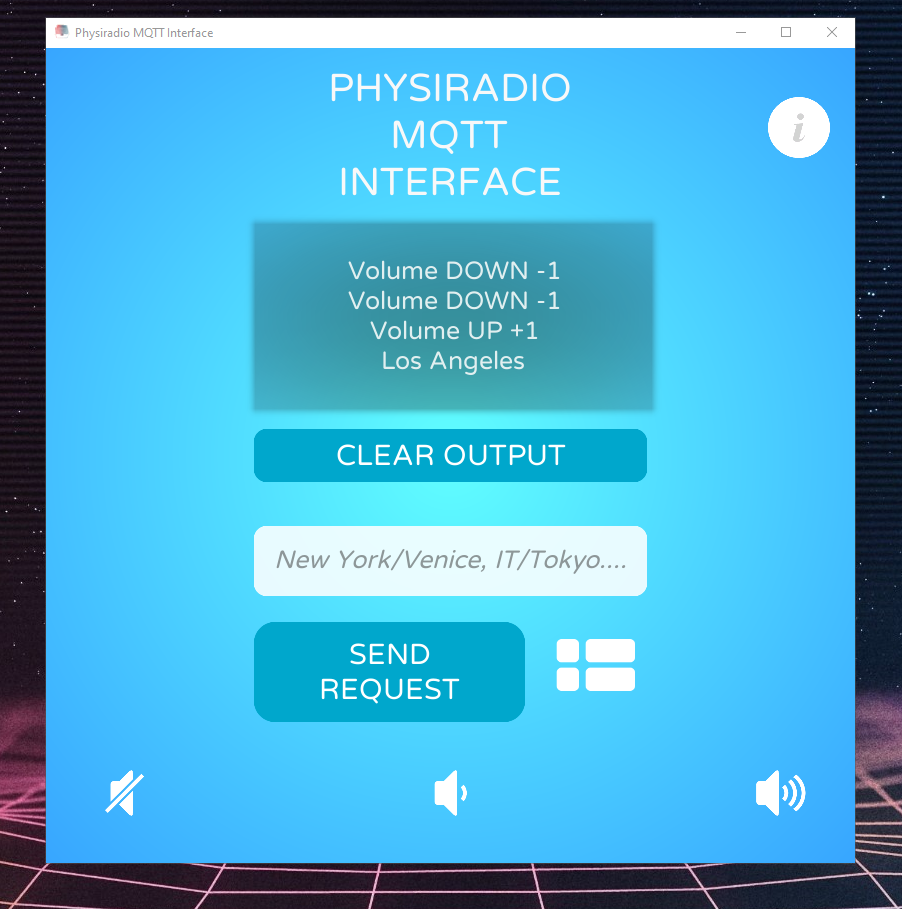
\includegraphics[width=.507\textwidth]{Immagini/screenshot_Physiradio_windows_1.png}
			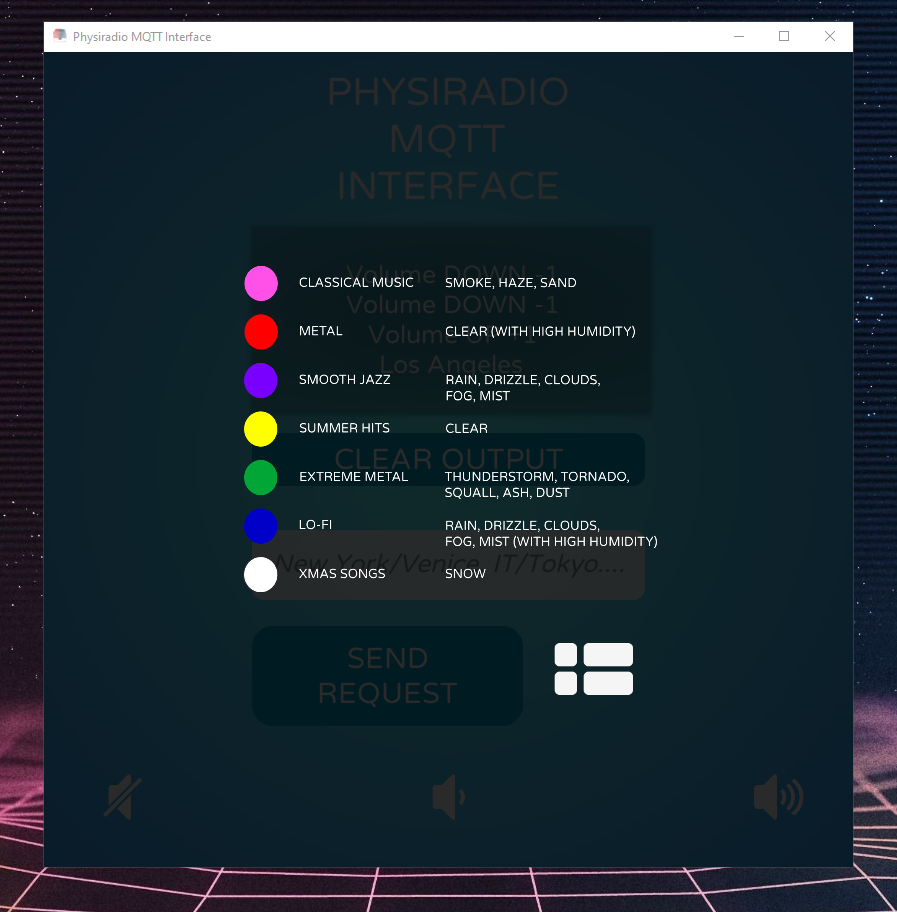
\includegraphics[width=.502\textwidth]{Immagini/screenshot_Physiradio_windows_2.png}
		}
		\caption{Physiradio MQTT Interface su Android(sotto) e Windows 10 (sopra)}
		
		\centerline
		{
			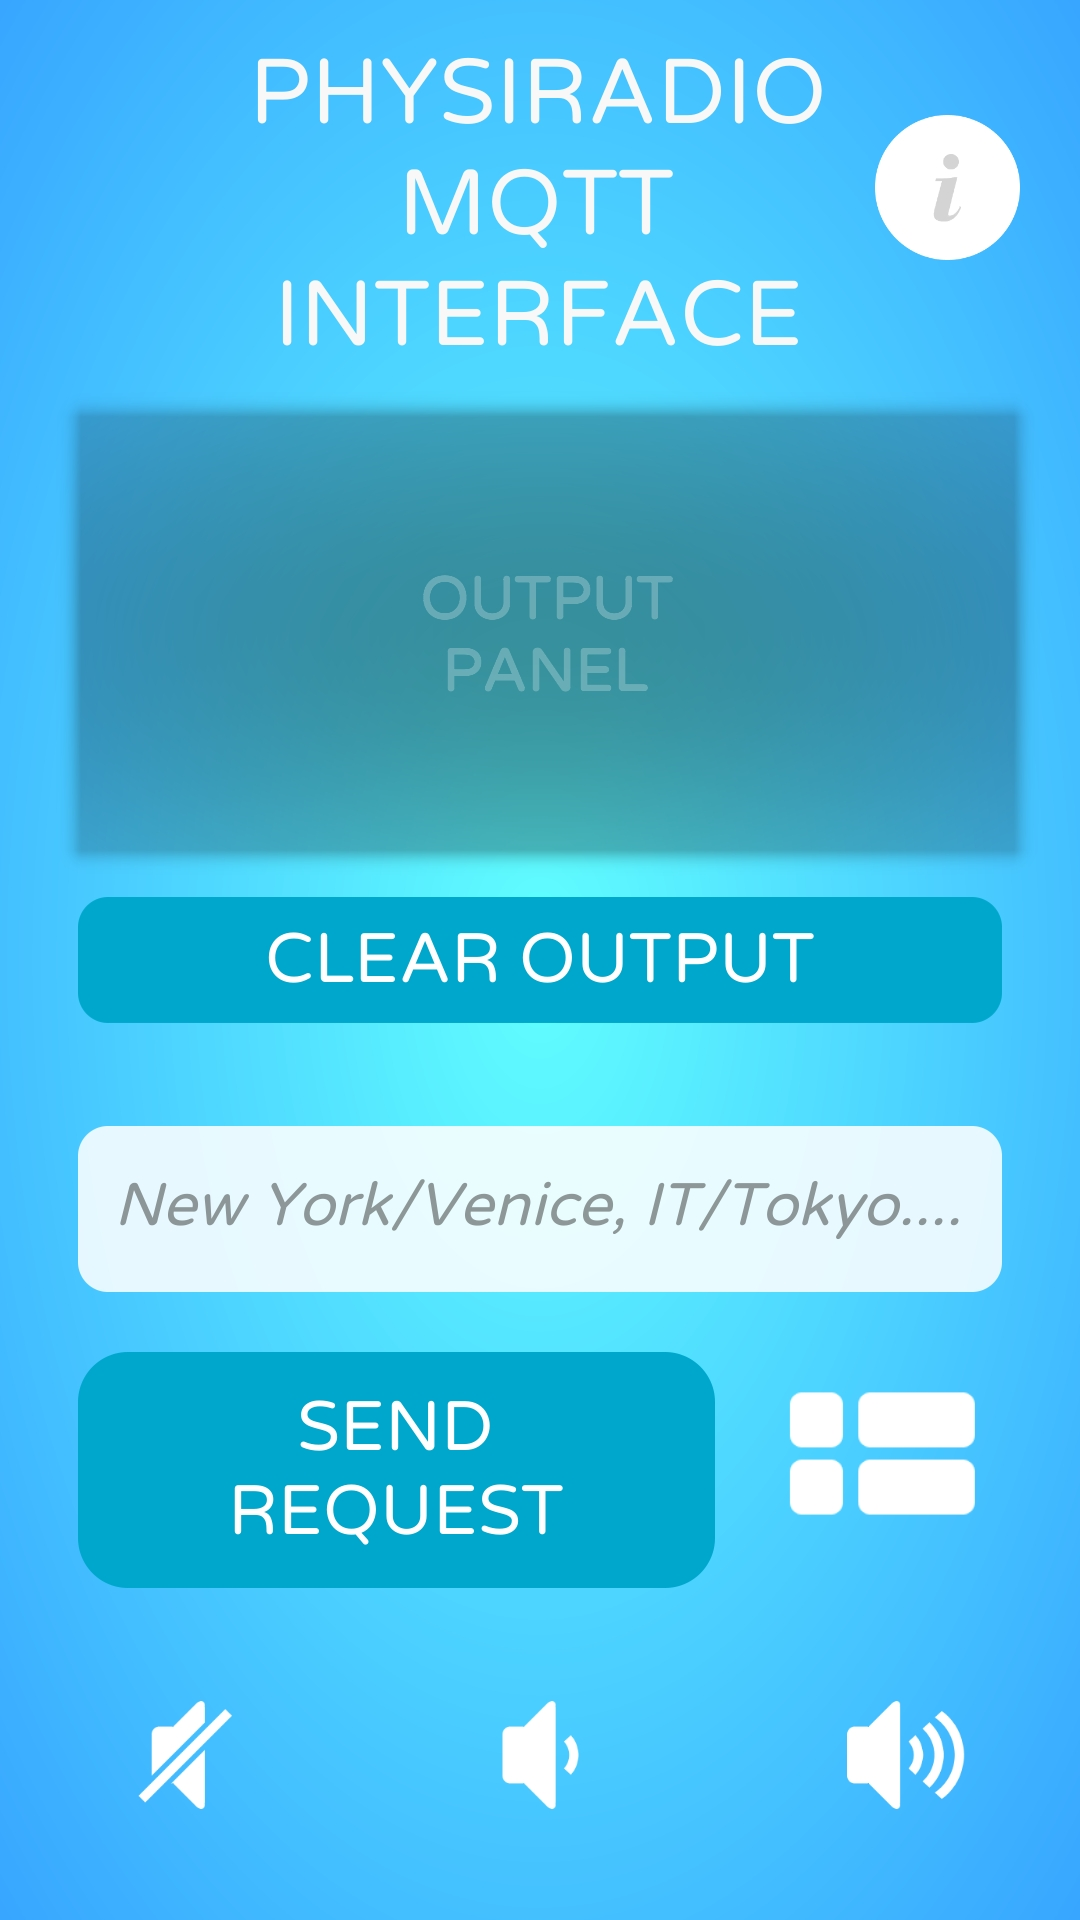
\includegraphics[width=.4\textwidth]{Immagini/physiradio_screenshot_android.jpg}
		}
		\label{fig:app}
	\end{center}
\end{figure}

\newpage
L'applicazione (Figura \ref{fig:app}) consiste di una singola schermata, da cui è possibile inviare messaggi MQTT a \physiradio, dello stesso formato descritto nel paragrafo precedente \ref{sec:descriptionInteraction}, e non solo. In particolare è possibile:
\begin{compactitem}
	\item Controllare il volume : mute/unmute, volume -1 e volume +1;
	\item Inviare una città da interrogare tramite le API di OpenWeatherMap: si compila il riquadro centrale bianco e si preme il bottone `SEND REQUEST';
	\item Visualizzare gli ultimi quattro comandi inviati al device IoT (utilizzando sempre QoS 0, di conseguenza non avremo mai la certezza dell'arrivo del messaggio);
	\item Visualizzare il riquadro delle informazioni (pulsante rotondo con la `i');
	\item Visualizzare una legenda sul mapping utilizzato (descritto nella sezione \ref{sec:mapping}) con colore visualizzabile della striscia led, genere musicale e tempo atmosferico. Visibile nel riquadro in alto a destra della Figura \ref{fig:app}.
\end{compactitem}
Sull'ultimo punto descritto, è necessario specificare che è una feature implementata al fine di aumentare la facilità di comprensione del device e del dato che in quel momento viene fisicalizzato, poiché, conferendo una legenda, l'utente non è più obbligato a interpretare la musica e i colori che vede, in funzione del dato che potrebbe rappresentare, ma gli basterà usufruire del device e, nel dubbio interpretativo, interrogare la legenda. Purtroppo, per limiti temporali e logistici, l'utilizzo dell'applicazione non è stata testata sugli utenti che si sono offerti per il \textit{field testing} del device.\\

Un nota importante da fare, è relativa alla libreria utilizzata per implementare il protocollo MQTT. Si tratta della libreria M2Mqtt\cite{mqttUnity} sviluppata da Ian Craggs, la quale permette di istanziare un client MQTT, il quale può connettersi ad un broker ed eseguire comandi sia di \textit{publish} che di \textit{subscribe}. Nel nostro caso, l'applicazione si limita solamente a pubblicare, poiché \physiradio\ non pubblica messaggi, perciò non vi è la necessità di sottoscrivere l'app a nessun topic.

\chapter{Field testing e analisi feedback}

Finita la preparazione del prototipo, lo step finale è stato quello di testarne l'esperienza di fruizione su un campione di persone, 59 per l'esattezza, al fine di raccogliere dati sull'esperienza provata nell'utilizzare \physiradio, e per capire se ha svolto il compito per il quale è stato creato. Ossia quello di poter far concepire il dato, proveniente da una sorgente \textit{open} (in particolare, il tempo atmosferico), tramite una fisicalizzazione che sfrutta il senso dell'udito, stimolato dalle canzoni, e la vista, tramite i colori dei led; e se gli utenti ne sono stati incuriositi.

\subsection{Somministrazione con questionario}

Nel dettaglio, per testare questa idea di musicalizzazione, è stato creato un questionario anonimo.
Sono state organizzate numerose sessioni di ascolto in cui studenti universitari, colleghi, amici, membri di hacklab locali e alcuni parenti, sono stati sottoposti alla fisicalizzazione di \physiradio, dalla quale hanno potuto suggerire molti spunti e conferire feedback importanti.\\
%\todo{atrent: borderei il questionario in modo da renderlo "avulso" dal testo della tesi, puoi usare un box di qualche genere, anche package techbox. simo: concordo}
Di seguito viene riportato il questionario per intero:\\
\newpage

%\hrule
%\medskip

%%%%inizio riquadro

\begin{mdframed}[leftmargin=-40pt,rightmargin=-40pt]

%INIZIO QUESITONARIO
%%%%%%%%%%%%%%%%%%%%%%%%%%%%%%%%%%%%%%%%%%%%%%%%%%%%%%%%%%%%%%%

\textit{Physiradio} è un dispositivo IoT (\textit{Internet of Things}) dimostrativo: recupera dalla rete i dati relativi alle condizioni meteo di un luogo scelto in fase di configurazione, li elabora e li rappresenta attraverso una combinazione di musica (genere musicale) e colore. Realizza cioè una possibile ``tangibilizzazione'' (liberamente tradotto dall'inglese \textit{physicalization}) di un dato.
%In particolare, a seconda del tempo atmosferico rilevato, verranno emessi uno specifico genere musicale e uno specifico colore dei led (sotto il prototipo).

\setlength\intextsep{0pt}
\begin{wrapfigure}{r}{0.4\textwidth} %prima era 0.3 ma col box funziona
	%\vspace{-50pt} % non va tolto!
	\begin{center}
		\includegraphics[width=0.35\textwidth]{Immagini/SCHEMA_PHYSIRADIO.png}
		%	\caption{Schema del dispositivo}
	\end{center}
\end{wrapfigure}


Lo scopo di questa demo è raccogliere impressioni su:
\begin{compactitem}
	\item l'idea di rappresentazione del dato atmosferico mediante musica e colori
	\item l'efficacia dello strumento nel sollevare curiosità sulla tecnica di estrazione del dato stesso
\end{compactitem}
\textbf{Nota bene}: non cerchiamo l'associazione perfetta, ci interessa valutare il procedimento di rappresentazione.
%
%%	\begin{figure}[hbt!]
%\begin{center}
%	\includegraphics[width=.4\textwidth]{SCHEMA_PHYSIRADIO.png}
%\end{center}
%%	\end{figure}

Ti chiediamo di compilare il questionario (anonimo) che segue, man mano che procediamo con la dimostrazione,
per fornirci un \textit{feedback} sul lavoro che stiamo realizzando.


\medskip
\hrule
\medskip

%\todo{atrent: preparare proprio il modulo come se fosse cartaceo (anche se poi magari lo compiliamo al pc)}
\begin{compactenum}
	\item Anagrafica (anonima):
	\begin{itemize}
		\item Età [\dots\dots] - Sesso F[~~]~~M[~~] - Città di residenza [\dotfill]
		\item Occupazione [\dotfill]
		\item Titolo di studio: Obbligo[~~]~~Superiori[~~]~~Laurea[~~]~~PhD[~~]
		\item Ascoltatore abituale di musica: Sì[~~]~~No[~~]
		\item Se ``Sì'':
		\begin{compactenum}
			
			\item Su quale \textit{device}?\newline
			Radio[~~]
			Webradio[~~]
			CD[~~]
			Vinile[~~]
			MP3~player~(o~smartphone~offline)[~~]
			App~streaming[~~]\medskip
			
			\item In che contesto?\newline
			Casa[~~]
			Lavoro[~~]
			Auto[~~]
			Mezzi~pubblici[~~]
			\newline
			Bagno[~~]
			Letto[~~]
			%			\newline
			Allenamento[~~]
			Passeggiando[~~]\newline
			Altro[\dotfill]\medskip
			
			\item Quali generi musicali ascolti?\newline
			[\dotfill]\newline
			[\dotfill]
		\end{compactenum} 
		
	\end{itemize}
	
	\item Ora ti faremo ``ascoltare e vedere'' alcune condizioni meteo senza dirti a cosa corrispondono, ti chiediamo per ogni ascolto di inserire uno a o più X in corrispondenza delle condizioni meteo che meglio lo rappresentano. 
	
\medskip
%\begin{table}[h]
	\begin{center}
	\centerline{\begin{tabular}{|c||c|c|c|c|c|c|c|c|c|c|c|c|c|c|c||c|} 
		\hline
		\textbf{Ascolto} &  \rotatebox{90}{\textbf{Pioggia}} & \rotatebox{90}{\textbf{Pioggerella}} & \rotatebox{90}{\textbf{Sereno/Soleggiato}} &  \rotatebox{90}{\textbf{Nuvoloso}} & \rotatebox{90}{\textbf{Temporale}} & \rotatebox{90}{\textbf{Uragano/Nubifragio}} & \rotatebox{90}{\textbf{Tornado}} & \rotatebox{90}{\textbf{Neve}} & 
		\rotatebox{90}{\textbf{Fumo}} & \rotatebox{90}{\textbf{Nebbia}} & \rotatebox{90}{\textbf{Foschia}} & \rotatebox{90}{\textbf{Caligine}} & \rotatebox{90}{\textbf{Sabbia}} & \rotatebox{90}{\textbf{Cenere}} & \rotatebox{90}{\textbf{Polvere}} & \rotatebox{90}{\textbf{Umidità (Rel.)$\geq$85\% }} \\
		\hline
		\hline
		Ascolto 1 & & & & & & & & & & & & & & & & \\
		\hline
		Ascolto 2 & & & & & & & & & & & & & & & &  \\
		\hline
		Ascolto 3 & & & & & & & & & & & & & & & & \\
		\hline
		Ascolto 4 & & & & & & & & & & & & & & & & \\
		\hline
		Ascolto 5 & & & & & & & & & & & & & & & & \\
		\hline
		Ascolto 6 & & & & & & & & & & & & & & & & \\
		\hline
		Ascolto 7 & & & & & & & & & & & & & & & & \\
		\hline 
	\end{tabular}}
	\end{center}
%\end{table} 

\medskip
\item Quale genere musicale e/o colore assoceresti alle seguenti condizioni meteo? (puoi anche compilarla parzialmente: inserisci almeno le associazioni che ti sembrano più calzanti; per aiutarti, puoi anche partire da un genere musicale e associare una condizione meteo)
\begin{compactitem}
	\item Nebbia [\dotfill]
	
	\item Pioggia [\dotfill]
	
	\item Pioggerella [\dotfill]
	
	\item Sereno/Soleggiato [\dotfill]
	
	\item Nuvoloso [\dotfill]
	
	\item Temporale [\dotfill]
	
	\item Uragano/Nubifragio [\dotfill]
	
	%\item Inquinato/Polveroso [\dotfill]
	
	\item Neve [\dotfill]
	

\end{compactitem}
	
	\item Ritieni efficace/utile la rappresentazione di questo tipo di dato tramite genere musicale e colore?
	
	%\hrulefill 
	~Poco[~~]~~Abbastanza[~~]~~Molto[~~]~~Moltissimo[~~]
	
	
	\item Ci suggeriresti un altro tipo di dato interessante da tangibilizzare con questo strumento?\newline
	[\dotfill]\newline
	[\dotfill]
	
	
	\item \textbf{Open Data}\newline
	I dati meteo usati in questo prototipo sono recuperati in tempo reale via rete da fonti cosiddette ``open data'', cioè fonti che forniscono informazioni liberamente utilizzabili tramite programmi (quindi non solo attraverso pagine web). Dentro Physiradio gira infatti un programma che recupera dati dalla rete e sceglie uno \textit{stream} musicale e un colore in base al \textit{mapping} che hai appena sperimentato.
	
	Lo scopo primario del processo di tangibilizzazione è quello di rendere fruibile i dati attraverso vari sensi, ma nel caso particolare di Physiradio ci interessa anche stimolare la curiosità sugli aspetti tecnologici del mondo dei dati aperti e della trasparenza, cioè:
	\begin{compactitem}
		\item Come vengono resi disponibili i dati e come si possono recuperare?
		\item Che forma hanno questi dati e che tipo di elaborazioni/visualizzazioni sono possibili?
	\end{compactitem}
	Ti abbiamo incuriosito?
	~~Poco[~~]~~Abbastanza[~~]~~Molto[~~]~~Moltissimo[~~]

\end{compactenum}

\hrulefill

\textbf{Commenti liberi:}

[\dotfill]

[\dotfill]

[\dotfill]

[\dotfill]

[\dotfill]

\hrulefill

\textbf{GRAZIE!}


\end{mdframed}


%%% fine riquadro
%FINE QUESITONARIO
%%%%%%%%%%%%%%%%%%%%%%%%%%%%%%%%%%%%%%%%%%%%%%%%%%%%%%%%%%%%%%%
 
\subsection{Analisi dei feedback}


Tutti i questionari sono stati analizzati singolarmente e sono stati registrati in un dataset. %\todo{simo to atrent: termine bruttino mi sa. atrent: registrati? simo: meglio}
Esso, disponibile tramite Zenodo \cite{datiQuestionario}, è stato elaborato tramite un notebook Jupyter\cite{jupyter} sul quale è stato creato uno script Python 3 che sfrutta principalmente la libreria Pandas\cite{pandasLib} per eseguire l'analisi dei dati.

Di seguito sono riportate le statistiche più rilevanti estratte dal dataset:
%\todo{atrent: valuterei la resa grafica di questi dati. simo: personalmente penso ci siano già molte rappresentazioni grafiche, ho riflettuto e non penso di mettere anche queste - atrent:ok}

\begin{compactitem}
	\item Proporzione Uomini/Donne: $78/22\%$;
	
	\item Età media: 30.5 anni (dev. std: 15.4);
	
	\item `Studente' è la classe più rappresentata con $64\%$, seguito da `Impiegato' $21\%$. `Pensionato', `Ricercatore', `Libero professionista' e altre classi non superano il $3\%$;
	
	\item Il $34\%$ vive a Milano, il resto del campione vive prevalentemente nella provincia di Milano, tutti in Lombardia tranne qualche sporadica eccezione che abita in Piemonte;
	
	\item Titoli di studio: Diplomati $67.8\%$, Laureati $22.1\%$, PhD $8.4\%$, Scuola dell'obbligo $1.7\%$ ;
	
	\item Il $96.6\%$ del campione è un ascoltatore abituale di musica, dei quali:
	\begin{compactitem}
		
		\item Contesto di ascolto: `Casa' $22\%$, `Auto' $18\%$, `Mezzi pubblici' $18\%$, `Passeggiando' $12\%$, `Allenamenti' $8.3\%$, `Letto' $8\%$, `Bagno' $6.5\%$ , `Lavoro' $4.6\%$, gli altri contesti non superano il $4\%$.
		
		\item Dispositivo di ascolto: `App streaming musicale' $33.3\%$, `Lettore MP3' $23.9\%$, `Radio' $18.8\%$, `CD' $12.8\%$, `Vinile' $6.8\%$ e `Webradio' $4.2\%$.\\
		
	\end{compactitem}
	
\end{compactitem}


\medskip
La Figura \ref{fig:effectiveness_and_curiosity} mostra i grafici a torta relativi alle risposte date dagli utenti sottoposti al questionario riguardanti l'efficacia soggettiva, rispetto al prototipo presentato, e a quanto sono stati incuriositi dall'oggetto stesso.\\

\bigskip

\begin{figure}[H]
	\begin{center}
		\def\angle{175}
		\def\radius{3}
		\def\cyclelist{{"blue","red","yellow","green"}}
		\newcount\cyclecount \cyclecount=-1
		\newcount\ind \ind=-1
		\resizebox{.99\textwidth}{!}{
			\begin{tikzpicture}[nodes = {font=\sffamily}]
			\foreach \percent/\name in {
				11.9/Poco,
				44.1/Abbastanza,
				40.7/Molto,
				3.3/Moltissimo
			} {
				\ifx\percent\empty\else             % If \percent is empty, do nothing
				\global\advance\cyclecount by 1     % Advance cyclecount
				\global\advance\ind by 1            % Advance list index
				\ifnum3<\cyclecount                 % If cyclecount is larger than list
				\global\cyclecount=0              	% reset cyclecount and
				\global\ind=0                     	% reset list index
				\fi
				\pgfmathparse{\cyclelist[\the\ind]} % Get color from cycle list
				\edef\color{\pgfmathresult}         %   and store as \color
				% Draw angle and set labels
				\draw[fill={\color!50},draw={\color}] (0,0) -- (\angle:\radius)
				arc (\angle:\angle+\percent*3.6:\radius) -- cycle;
				\node at (\angle+0.5*\percent*3.6:0.7*\radius) {\percent\,\%};
				\node[pin=\angle+0.5*\percent*3.6:\name]
				at (\angle+0.5*\percent*3.6:\radius) {};
				\pgfmathparse{\angle+\percent*3.6}  % Advance angle
				\xdef\angle{\pgfmathresult}         %   and store in \angle
				\fi
			};
			\node [font=\large\bfseries] at (0, 5) {Efficacia};
			\end{tikzpicture}
			
			\begin{tikzpicture}[nodes = {font=\sffamily}]
			\foreach \percent/\name in {
				3.4/Poco,
				30.5/Abbastanza,
				49.2/Molto,
				16.9/Moltissimo
			} {
				\ifx\percent\empty\else             % If \percent is empty, do nothing
				\global\advance\cyclecount by 1     % Advance cyclecount
				\global\advance\ind by 1            % Advance list index
				\ifnum3<\cyclecount                 % If cyclecount is larger than list
				\global\cyclecount=0              	% reset cyclecount and
				\global\ind=0                     	% reset list index
				\fi
				\pgfmathparse{\cyclelist[\the\ind]} % Get color from cycle list
				\edef\color{\pgfmathresult}         % and store as \color
				% Draw angle and set labels
				\draw[fill={\color!50},draw={\color}] (0,0) -- (\angle:\radius)
				arc (\angle:\angle+\percent*3.6:\radius) -- cycle;
				\node at (\angle+0.5*\percent*3.6:0.7*\radius) {\percent\,\%};
				\node[pin=\angle+0.5*\percent*3.6:\name]
				at (\angle+0.5*\percent*3.6:\radius) {};
				\pgfmathparse{\angle+\percent*3.6}  % Advance angle
				\xdef\angle{\pgfmathresult}         %   and store in \angle
				\fi
			};
			
			%\node[above,font=\large\bfseries] at (current bounding box.south) {Curiosità};
			\node [font=\large\bfseries] at (0, 5) {Curiosità};
			\end{tikzpicture}
			
		}
		
		\caption{Risposte date riguardanti l'efficacia (sinistra) dell'attuale prototipo e la curiosità instillata (destra). 
			In basso invece si possono analizzare le statistiche relative ai due dati sopra citati (per poter generare una statistica sulla valutazione (a risposta chiusa) di ogni utente, è stato eseguito un mapping, dell'intervallo Poco$\rightarrow$Moltissimo, con numeri interi da 1 a 4)}
		\label{fig:effectiveness_and_curiosity}
		
		\bigskip
		
		\begin{tabular}[h]{|c|c|c|c|c|c|c|}
			\hline
			\textbf{} & \rotatebox{90}{\textbf{Poco (1)}} & \rotatebox{90}{\textbf{Abbastanza (2)}} & \rotatebox{90}{\textbf{Molto (3)}} & \rotatebox{90}{\textbf{Moltissimo (4)}} & \textbf{Media} & \textbf{Dev.Std} \\
			\hline
			Efficacia & 11.9\% & 44.1\% & 40.7\% & 3.3\% & 2.35 & 0.73 \\  %0.119 & 0.441 & 0.407 & 0.033 & 2.35 & 0.73
			\hline
			Incuriosito & 3.4\% & 30.5\% & 49.5\% & 16.9\% & 2.79 & 0.76 \\  %0.034 & 0.305 & 0.495 & 0.169 & 2.79 & 0.76
			\hline
		\end{tabular}
		
	\end{center}
\end{figure} 


L' \textbf{indice di correlazione} tra \textit{Incuriosito} e l'\textit{Efficacia} è di $0.47$ (con covarianza $0.26$),
%Indice di correlazione Incuriosito-Efficacia 	  0.46950013744344243
%Covarianza Incuriosito-Efficacia 		  0.26329631794272357
%
tra \textit{Età} e \textit{Incuriosito} è di $-0.0039$ (con covarianza $-0.46$),
%Indice di correlazione Eta-Incuriosito	  -0.003949642980854196
%Covarianza Eta-Incuriosito 		  -0.046464056107539405
%
tra \textit{Età} e \textit{Efficacia} è di $0.012$ (con covarianza $-0.14$).
%Indice di correlazione Eta-Efficacia	  -0.012148290838946635
%Covarianza Eta-Efficacia 		  -0.13851548801870206

Possiamo notare che la correlazione tra fattore di curiosità accresciuta e l'efficacia del dispositivo è di circa 0.5. Questo ci suggerisce che i due valori sono abbastanza legati fra di loro da una leggera relazione lineare: una buona parte di chi è stato convinto dalla funzionalità dell'oggetto è stato anche genuinamente incuriosito da come funzionasse. \\
Inoltre, dalle statistiche estratte, si evince che, il fatto di ritenere il device efficace e di esserne stati incuriositi, non ha pressoché alcuna rilevanza rispetto all'età degli utenti. Da questo punto di vista il campione è omogeneo.\\


Oltre a chiedere l'opinione degli utenti, l'efficacia della mappatura è stata anche misurata verificando le corrispondenze tra l'ascolto e le condizioni meteorologiche associate. La Figura \ref{fig:matches_total} elenca e traccia le frequenze corrispondenti \footnote{I valori vanno da $0\%$ (nessuno ha `indovinato') a $100\%$ (tutti hanno `indovinato').} per ogni ascolto riprodotto. I valori mostrano che gli ascolti 4, 5, 6 e 7 sono stati `indovinati' correttamente molto spesso, mentre gli ascolti 1, 2 e 3 sono stati associati correttamente di rado.\\ 

\begin{figure}[H]
	\begin{center}
		\centerline{\begin{tabular}{|l l|l| }
				\hline
				& & \\
				Ascolto n.1 & 0.00\%  & \multirow{7}{*}{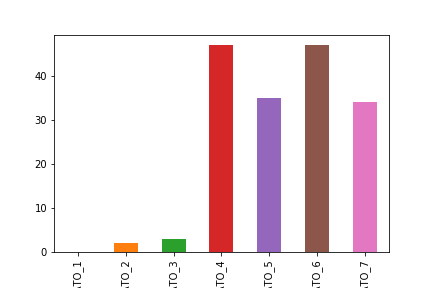
\includegraphics[width=.40\textwidth]{../Questionario/total_barplot.png}\bigskip}  \\ %dimensione già calcolata per versione finale
				%			\hline 
				Ascolto n.2 & 3.38\%   & \\ 
				%	0.03		\hline 
				Ascolto n.3 & 5.08\%   & \\
				%	0.05		\hline 
				Ascolto n.4 & 79.66\%  & \\ 
				% 0.79			\hline 
				Ascolto n.5 & 59.32\%  & \\ 
				%	0.59		\hline 
				Ascolto n.6 & 79.66\%  & \\
				%	 0.79		\hline 
				Ascolto n.7 & 57.62\%  & \\ 
				% 0.57
				& & \\
				\hline 
		\end{tabular}}
		\caption{Conteggio delle corrispondenze trovate tra il valore dato dagli utenti per ogni ascolto e l'effettivo valore associato dal mapping (ricordiamo che il campione è di 59 utenti)}
		\label{fig:matches_total}
	\end{center}
\end{figure}

Questi dati in realtà non sorprendono molto, da come si poteva già notare nella tabella \ref{tab:mapping}, i tempi atmosferici legati agli ascolti n.1, 2, e 3, sono quelli di cui ci si aspettava una più difficile interpretazione. In primo luogo, i generi musicali assegnati sono, purtroppo, molto ampi come spettro di sonorità. Secondariamente, quegli specifici tempi atmosferici erano i più complessi da rappresentare. Analizzando i due paper di riferimento \cite{karmaker2015automated} e \cite{predictingmoodonmusicgenre} si nota innanzitutto che le condizioni `Fumo',`Caligine' e `Sabbia' non sono neanche stati citati, mentre potrebbero comunque essere ricevuti da OpenWeatherMap, di conseguenza la scelta del genere è stata complessa e, purtroppo, fallimentare. Successivamente, per quanto riguarda l'ascolto n.2, il tempo atmosferico `Sereno con molta umidità', assimilabile come afa, non è quasi mai stato preso in considerazione dal campione di utenti, forse perché poco comune e non molto intuitivo rispetto al semplice `Sereno'. Lo stesso principio vale per l'ascolto n.3, ma al contrario; probabilmente l'utente medio percepisce i tempi come `Pioggia', `Pioggerella', `Foschia' ecc\dots direttamente con un alto tasso di umidità invece che considerare anche il caso in cui sia bassa.

%\todo{simo to atrent : spiegare il perché? atrent: si. simo: ho provato cosí - atrent:ok}



\chapter{Conclusioni e futuri sviluppi}\label{sec:conclusions}

I risultati mostrano che \physiradio\ è ben accettato dall'utenza che ne ha usufruito (letteralmente ``che bell'oggetto!" è stato affermato frequentemente) e che stimola efficacemente la curiosità sui funzionamenti interni e sui dati aperti: il $66.1\% $ (Figura \ref{fig:effectiveness_and_curiosity}) dei soggetti ha indicato $Molto$ o $Moltissimo$ sulla sezione riguardo l' ``aumento della curiosità'', e non vi è correlazione per età a riguardo. \\ %\todo{atrent: sugli ``interni'' non si dice. simo: sui funzionamenti interni meglio?} 
Coloro che lo hanno trovato interessante, hanno anche assegnato un valore ``relativamente alto''\footnote{+0.5 è la soglia per cui iniziare ad a tenere in considerazione la correlazione, citando https://www.dummies.com/education/math/statistics/how-to-interpret-a-correlation-coefficient-r/} per l'efficacia (correlazione: $0,47$). \\%\todo{in realtà non è altissima, puoi dire "relativamente alta" e spiegare perché, cfr. https://www.dummies.com/education/math/statistics/how-to-interpret-a-correlation-coefficient-r/} 
%\todo{simo to atrent: ti ho preso alla lettera, la spiegazione è stata data già sopra - atrent:ok}
Il $44\%$ dei soggetti ha dichiarato che il prototipo è molto efficace e che trova coerente la mappatura tra condizioni meteorologiche e la coppia genere musicale-colore. Questa valutazione è stata confermata analizzando le corrispondenze effettive (Figura \ref{fig:matches_total}) tra il mapping utilizzato e il mapping ipotizzato (musica e colore $\rightarrow$ tempo atmosferico) dagli utenti. In quattro ascolti (ovvero 4, 5, 6, 7) su sette, le corrispondenze sono state spesso ``indovinate'' (tra $59.32\% $ e $79.6\%$ delle volte), al contrario dei restanti tre ascolti (vale a dire 1, 2, 3) dove quasi mai (tra lo $0\%$ e $5.08\%$ delle volte) sono state individuate correttamente.\\

Un problema emerse molto presto: il genere musicale è una definizione troppo ampia \footnote{Ad esempio, un webradio ``latino'' potrebbe suonare ``salsa'', ``bachata'', ``reggaeton'', ``chacha'', ecc... che sono molto diversi tra loro. In effetti, in termini musicali, non esiste una definizione universalmente accettata di generi specifici.} da usare \textit{invertita}, ovvero estrapolando le condizioni meteorologiche originali partendo dal genere. Inoltre, l'associazione tra musica, colori, e clima è, ovviamente, molto soggettiva; specialmente se come nesso hanno l'umore/\textit{mood} indotto nell'utente. \\
Sebbene il processo di \textit{musicalization} soddisfi il presupposto di essere una ``sonificazione'' formale (cioè, stessa condizione meteorologica $\rightarrow$ stesso genere musicale), è anche vero che il genere potrebbe non essere sufficiente, per tutti i fruitori, al fine di associare una specifica condizione meteorologica, anche con l'aiuto del colore \footnote{Non tutti i soggetti hanno notato / utilizzato i LED colorati, a volte perché l'ambiente non aveva un'illuminazione adeguata (ad es. troppa luce ambientale) e talvolta perché il soggetto ha deciso (e dichiarato) di non prestare attenzione a entrambe, musica e luce.}. \\
Difatti, tutte le webradio utilizzate sono incentrate su un genere specifico, ciò nonostante risulta comunque vasta la gamma di brani appartenenti allo stesso genere. Perciò le sessioni sperimentali effettive, sono state in qualche modo influenzate dal brano riprodotto in quel preciso lasso di tempo, e molto probabilmente, ripetendo i test in altri momenti, i risultati sarebbero potuti essere differenti.\\ 
Un suggerimento molto importante ricevuto da un collega è stato il seguente: ``invece di utilizzare una webradio incentrata sul genere per ogni canale di streaming, sarebbe meglio creare playlist specifiche, meglio se definite dall'utente''. Ad esempio, ogni utente di \physiradio\, a lungo termine, dovrebbe essere in grado di personalizzare la sua configurazione in termini di:
\begin{compactitem}
	\item Che tipo di dato potrebbe essere preso in input;
	\item Creare playlist customizzabili;
	\item Associare quelle playlist a dei valori enumerabili.
\end{compactitem}
In realtà, questa opzione è stata prevista nella progettazione: l'adozione di MQTT come linguaggio di interfaccia per controllare il dispositivo, è stata scelta per facilitare l'integrazione con sistemi come IFTTT \cite{ifttt}, con un Connettore MQTT, oppure Node-RED \cite{nodeRed}, pronto per MQTT. \physiradio\ può essere completamente controllato tramite un'API MQTT con comandi come `volume ',`stazione', `città'(per ottenere dati meteorologici specifici), ecc. In questo modo, anche un utente semi-tecnico\footnote{Sia IFTTT che NodeRED sono molto facili da usare e intuitivi.} potrebbe implementare una configurazione adatta.


Naturalmente, la soluzione più semplice al ``problema della soggettività'' sarebbe quella di descrivere la mappatura nella documentazione (o tramite un piccolo display) in modo che una volta assimilata, nessun utente debba impegnarsi ad interpretare il dispositivo in seguito. Problema che è stato in parte risolto introducendo una legenda all'interno dell'app sviluppata con Unity (Figura \ref{fig:app} in alto a destra). \\ 


Altri consigli ricevuti, per quanto riguarda la diminuzione della soggettività a favore dell'oggettività, sono stati:
\begin{compactitem}
	\item Utilizzare musiche per balli molto più canonizzate (ad esempio `salsa', `tango', `can can', `tarantella' ecc...) probabilmente abbasserebbero il grado di soggettività o limiterebbero il problema della difficoltà nel definire un genere musicale.	
	\item Sfruttare meglio le luci e i colori, per esempio far pulsare i LED a ritmo, seguendo il tempo del brano. \\
\end{compactitem}


Durante le sessioni sperimentali, molti soggetti sono stati ispirati dal dispositivo e hanno iniziato a suggerire altre mappature basate sul loro lavoro e sulla loro esperienza di vita, come:

\begin{compactitem}
\item Carico complessivo della CPU (in una server farm);

\item Traffico di rete, non solo in termini di volume ma anche in termini di tipo di traffico (attacchi denial of service, spamming della posta con molti messaggi ripetuti, ecc\dots);

\item Condizioni del traffico cittadino;

\item Orari dei treni e ritardi (ad esempio ``Se devi uscire di casa al momento giusto, ma ti stai radendo/facendo il bagno/ecc.'');

\item Tempi di cottura (ad esempio ``Se hai voglia di un timer da forno musicale'');

\item Tempi di attesa del call center (musica che rappresenta il tempo di attesa di un operatore);

\item Vari contesti in cui sono coinvolti  dei bambini, i quali sono mediamente più sensibili alla musica e ai colori rispetto ad un'utenza adulta.

\end{compactitem}

\bigskip

In generale, qualsiasi situazione in cui vi è necessità di monitorare continuamente una `variabile'(dato), risulta utile sfruttare il potere di discernimento ``superiore'' (in termini di riconoscimento del cambio di stato) dell'ascolto rispetto alla vista \cite{10.1117/12.19981}. Inoltre, risulterebbe fastidioso e/o noioso rappresentare la variazione di stato con un tono/suono semplice, proprio per questo \physiradio\ risulta essere un mezzo utile ed interessante. \\

\bigskip

Come accennato precedentemente nella sezione \ref{sec:descriptionInteraction} e in altri paragrafi, le implementazioni future possibili riguardanti il software sono molteplici:
\begin{compactitem}
	\item Avendo creato il prototipo affinché interpreti i dati sul meteo in formato JSON, è possibile prendere in input dati/dataset differenti nello stesso formato, senza dover modificare troppo il codice. Magari anche dando la possibilità di scegliere dinamicamente quali fisicalizzare;
	\item Il mapping scelto è totalmente modificabile e aperto a chi volesse variarlo e migliorarlo;
	\item Il protocollo MQTT implementato potrebbe essere migliorato da più punti di vista. In prima istanza si possono implementare funzioni di \textit{subscribe}, sia da parte dello script che gira sul device sia per l'applicazione, al fine di migliorare l'interazione tra le due parti. Successivamente si possono pensare migliorie per quanto riguarda la suddivisione in \textit{subtopic} più specifici, divisi in classi, in modo da evitare una comunicazione ``\textit{broadcast}'' poco selettiva. O ancora, si potrebbe modificare il codice affinché acquisisca un livello di sicurezza maggiore, utilizzando QoS di livelli più alti dello 0 (il più basso).\\
\end{compactitem}

\bigskip
\newpage
Riassumendo, gli esperimenti sul campo sono stati molto soddisfacenti: i soggetti sono diventati molto loquaci e hanno posto molte domande.\\ La mappatura non è risultata molto efficace, ma rimane un dato relativo, poiché l'obiettivo principale dell'esperimento era creare un prototipo di device IoT che, fisicalizzando dei dati (open data nello specifico), tramite una combinazione di musica (genere musicale) e colore, stimolasse curiosità e immaginazione nell'utente, cosa che riesce a fare con successo.
Ultimo ma non meno importante, il design vintage del cabinet di legno scelto per il prototipo, si è rivelato una chiave di successo per l'accettazione del dispositivo da parte degli utenti.


\chapter*{Ringraziamenti}
Per prima cosa, vorrei ringraziare il Prof. Andrea Trentini per avermi aiutato nello sviluppo di questo progetto; è raro trovare professori così disponibili, umanamente buoni e competenti allo stesso tempo.\\
Un ringraziamento speciale va a Claudio, Cristina e Chiara, la mia famiglia, a cui devo tutto. Senza il loro sostegno  e il loro affetto, specialmente nei momenti di sconforto e difficoltà, probabilmente non sarei riuscito a completare questo percorso di studi. Sono orgoglioso di essere vostro figlio e fratello.\\
Ci terrei inoltre a ringraziare i miei compagni di studi Carlo, Noah, Stefano, Marco (D.N.), Alberto, Daniele e Marco (V.V.), con i quali ho condiviso momenti importanti della mia vita e della mia formazione.\\
Un saluto speciale va a tutti i componenti degli Elkir, la mia band nonché seconda famiglia, con cui ho portato avanti una splendida esperienza di vita in parallelo all'università e che spero duri il più possibile. \\
Infine ringrazio tutti i miei amici, vecchi e nuovi, che mi hanno sempre sostenuto e mi vogliono bene, a cui io stesso tengo moltissimo.\\
Grazie

%%%%%%%%%%%%%%%%%%%%%%%%% APPENDICE

\appendix
\chapter{Codice implementazione protocollo MQTT} \label{app:pubsub}

\begin{lstlisting}[style=customC++Arduino, label={Codice 1.1}, caption={Codice 1.1}, title={Codice 1.1: libreria PubSubClient}, basicstyle=\linespread{0.7}\footnotesize\ttfamily] 
#include <PubSubClient.h>
...
WiFiClient mqttClient; //ESP8266WiFi network client
PubSubClient psclient(mqttClient);

//Callback function for MQTT protocol
void mqttCallback(char* topic, byte* payload, unsigned int length); 
...
void setup () {
...
//MQTT setup
psclient.setServer("mqtt.atrent.it", 1883); //server name, port 
psclient.setCallback(mqttCallback);
reconnect();
...
}

void mqttCallback(char* topic, byte* payload, unsigned int length) {

	//Parsing the payload
	char msg[length];
	for (int i = 0; i < length; i++) {
	msg[i] = (char)payload[i];
	}
	//Adding EOF to cast msg to a string
	msg[length] = '\0';
	
	if(strcmp(topic, "PhysiRadio/Volume") == 0) {
	if(strcmp(msg, "mute") == 0) {
	Serial.println("Muting volume");
	player.setVolume(0);
	Serial.println("VOLUME : 0");
	}
	
	if(strcmp(msg, "unmute") == 0) {
	Serial.println("UnMuting volume");
	player.setVolume(TMP_VOLUME);
	Serial.print("VOLUME : ");
	Serial.println(TMP_VOLUME);
	}
	
	if(strcmp(msg, "+1") == 0) {
	Serial.println("Volume +1");
	TMP_VOLUME+=1.0;
	if (TMP_VOLUME <= 100.0) {
	player.setVolume(TMP_VOLUME);
	} else {
	TMP_VOLUME = 100.0;
	}
	VOLUME = TMP_VOLUME;
	Serial.print("VOLUME : ");
	Serial.println(TMP_VOLUME);
	}
	
	if(strcmp(msg, "-1") == 0) {
	Serial.println("Volume -1");
	TMP_VOLUME-= 1.0;
	if(TMP_VOLUME >= 0.0) {
	player.setVolume(TMP_VOLUME);
	} else {
	TMP_VOLUME = 0.0;
	}
	VOLUME = TMP_VOLUME;
	Serial.print("VOLUME : ");
	Serial.println(TMP_VOLUME);
	}
	}
	
	if(strcmp(topic, "PhysiRadio/Station") == 0) {
	
	if(strcmp(msg, "enable") == 0) {
	t_api.enable();
	Serial.println("API task Enabled");
	}
	
	if(strcmp(msg, "disable") == 0) {
	t_api.disable();
	Serial.println("API task Disabled");
	}
	
	if(strcmp(msg, "station1") == 0) {
	Serial.println(msg);
	Serial.println("Radio 1 - Classical -> Smoke/Haze");
	connect_radio(&radioClassical);
	}
	
	if(strcmp(msg, "station2") == 0) {
	Serial.println(msg);
	Serial.println("Radio 2 - Metal -> Clear(sun) + High humidity");
	connect_radio(&radioMetal);
	}
	
	if(strcmp(msg, "station3") == 0) {
	Serial.println(msg);
	Serial.println("Radio 3 - SmoothJazz -> Rain/Drizzle/Cloud/Fog  + low humidity");
	connect_radio(&radioSmoothJazz);
	}
	
	if(strcmp(msg, "station4") == 0) {
	Serial.println(msg);
	Serial.println("Radio 4 - SummerHits -> Sunny + low humidity");
	connect_radio(&radioSummer);
	}
	
	if(strcmp(msg, "station5") == 0) {
	Serial.println(msg);
	Serial.println("Radio 5 - ExtremeMetal -> Thunderstorm/Tornado...");
	connect_radio(&radioExtremeMetal);
	}
	
	if(strcmp(msg, "station6") == 0) {
	Serial.println(msg);
	Serial.println("Radio 6 - LoFi -> Rain/Drizzle/Cloud/Fog  + High humidity");
	connect_radio(&radioLoFi);
	}
	
	if(strcmp(msg, "station7") == 0) {
	Serial.println(msg);
	Serial.println("Radio 7 - Xmas Songs -> Snow");
	connect_radio(&radioXmas);
	}
	}
	
	//MQTT dynamic city change for API request
	if(strcmp(topic, "PhysiRadio/City") == 0) {
	cityRequested = String(msg);
	}
}

void reconnect() {

	//If it's not connected, try to connect
	if (!psclient.connected()) {
		Serial.print("Attempting MQTT connection...");
		
		//Attempt to connect
		if (psclient.connect(clientId.c_str())) {
		Serial.println(clientId + " connected to MQTT server");
		
		//Subscribe to all subtopics
		psclient.subscribe("PhysiRadio/#");
		
		} else {
		Serial.print("failed, rc=");
		Serial.print(psclient.state());
		}
	}
}

\end{lstlisting}

\chapter{Codice implementazione cooperative multitasking} \label{app:task}

\begin{lstlisting}[style=customC++Arduino, label={Codice 1.2}, caption={Codice 1.2}, title={Codice 1.2 : libreria TaskScheduler}, basicstyle=\linespread{0.7}\footnotesize\ttfamily]
#include <TaskScheduler.h>
...
//One WiFi client for each task, to garantee more connection stability
WiFiClient api;
WiFiClient music;
WiFiClient mqttClient;
...
//Scheduler and tasks definition
Scheduler scheduler;
void task_apiCallback();
void task_audioStreamCallback();
void task_mqttCallback();
...
//Call weather api function, every 10s
Task t_api(10 * TASK_SECOND, TASK_FOREVER, &task_apiCallback); 
//Call audio stream task, always(the minimum interval possible)
Task t_stream(0, TASK_FOREVER, &task_audioStreamCallback);
//Call mqtt callback to get mqtt messages, every 100ms
Task t_mqtt(100, TASK_FOREVER, &task_mqttCallback);            
...
void setup () {
	...
	//Scheduling tasks
	scheduler.init();
	Serial.println("Initialized scheduler");
	
	scheduler.addTask(t_api);
	Serial.println("added api task");
	scheduler.addTask(t_stream);
	Serial.println("added stream task");
	scheduler.addTask(t_mqtt);
	Serial.println("added mqtt task");
	
	t_api.enable();
	Serial.println("Enabled api task");
	t_stream.enable();
	Serial.println("Enabled stream task");
	t_mqtt.enable();
	Serial.println("Enabled mqtt task");
	...
}

//Just runs the scheduler 
void loop(){  
	scheduler.execute();
}
...
//Task for http get : OpenWeatherMap API -> returns JSON
void task_apiCallback() {
	if (!api.connect("api.openweathermap.org", 80)) {
	Serial.println("Connection failed");
	api.stop();
	return;
	}
	Serial.println("Connected to API domain!");
	//Send HTTP GET request
	String httpMsg = 
	String("GET /data/2.5/weather?q=" +
	cityRequested + 
	"&APPID=caaaf9c4e90fc42fe0baa94b8f1f6928&units=metric HTTP/1.0");
	Serial.println(httpMsg);
	api.println(httpMsg);
	api.println("Host: api.openweathermap.org");
	api.println("Connection: close");
	if (api.println() == 0) {
	Serial.println("Failed to send request");
	api.stop();
	return;
	}
	
	//Check HTTP status
	char status[32] = {0};
	api.readBytesUntil('\r', status, sizeof(status));
	if (strcmp(status, "HTTP/1.1 200 OK") != 0) {
	Serial.print("Unexpected response: ");
	Serial.println(status);
	api.stop();
	return;
	}
	
	//Skip HTTP headers
	char endOfHeaders[] = "\r\n\r\n";
	if (!api.find(endOfHeaders)) {
	Serial.println("Invalid response");
	api.stop();
	return;
	}
	
	//Allocate the JSON document 
	const size_t capacity = JSON_ARRAY_SIZE(4) + 
	2*JSON_OBJECT_SIZE(1) + 
	2*JSON_OBJECT_SIZE(2) + 
	4*JSON_OBJECT_SIZE(4) + 
	JSON_OBJECT_SIZE(5) + 
	JSON_OBJECT_SIZE(6) + 
	JSON_OBJECT_SIZE(14) + 
	1816; 
	//(1816, is an empirical byte value,
	//to ensure enough space for the json document)
	DynamicJsonDocument doc(capacity);
	
	//Parse JSON object
	DeserializationError error = deserializeJson(doc, api);
	if (error) {
	Serial.print("deserializeJson() failed: ");
	Serial.println(error.c_str());
	api.stop();
	return;
	}
	
	//Extract values
	JsonObject weather_0 = doc["weather"][0];
	JsonObject main_0 = doc["main"];
	const char* weather_0_main_char = weather_0["main"]; //eg "Clouds"
	const char* city_name_char = doc["name"]; //eg "Milan"
	city_name = String(city_name_char);
	weather_0_main = String(weather_0_main_char);
	humidity = main_0["humidity"];
	
	Serial.println("Response:");
	Serial.println(city_name);
	Serial.println(weather_0_main);
	Serial.print(humidity);
	Serial.println(" % humidity");
	
	//Execute weather-radiostation mapping 
	doMapping(weather_0_main);
}

void task_audioStreamCallback() {
if(!music.connected()) {
	Serial.println("Reconnecting for audio stream...");
	if(music.connect(httpHost, httpPort)) {
	music.print(String("GET ") + httpPath + " HTTP/1.1\r\n" +
	"Host: " + httpHost + "\r\n" +
	"Connection: close\r\n\r\n");
	Serial.println("connected to stream source");
	}
	}
	
	//Play stream
	if(music.available() > 0) {
	uint8_t bytesread = music.readBytes(mp3buff, BUFF);
	player.playChunk(mp3buff, bytesread);
	}
	
	//Code to control Physiradio easily by Serial input on Arduino IDE
	if (Serial.available() > 0) {
	// read the incoming byte for serial input control;
	incomingByte = Serial.read();
	switch(incomingByte) {
	... //VARI CASE PER IL CONTROLLO DEL DEVICE
	}
	}
}

void task_mqttCallback() {
	//Connect if we're not already connected.
	if (!psclient.connected()) reconnect();
	
	//Process any events.
	psclient.loop();
}

//Callback assigned to all mqtt clients
void mqttCallback(char* topic, byte* payload, unsigned int length) {
	//VEDERE SEZIONE SUL PROTOCOLLO MQTT
}

void reconnect() {
	//VEDERE SEZIONE SUL PROTOCOLLO MQTT
}

void doMapping(String weather) {
	if(weatherMap->has(weather)) {
	Serial.println("Doing mapping for " + weather + " weather");
	
	radioStation tempRadio = weatherMap->get(weather);
	
	//Cases for high humidity levels 
	if(humidity >= 85) { //
	if ( (tempRadio.name).equals(radioSummer.name) ) {
	tempRadio = radioMetal;
	}
	
	if( (tempRadio.name).equals(radioSmoothJazz.name) ) {
	tempRadio = radioLoFi;
	}
	}
	
	Serial.print("Got: " + tempRadio.name + " --> " );
	
	//If new radio is different from the actual, then connect
	//look host OR port, because some radios use
	//same host for multiple web radio switching on ports
	if((strcmp((tempRadio.host), httpHost) != 0) | (tempRadio.port != httpPort) ) {
	connect_radio(&tempRadio);
	} else {
	Serial.println("Already on the same station");
	}
	
	} else {
	Serial.println("Weather not mapped");
	}
}

void connect_radio(radioStation *radio) {
	fade_out_audio();
	
	httpHost = radio->host;
	httpPath = radio->path;
	httpPort = radio->port;
	
	if (!music.connect(httpHost, httpPort)) {
	Serial.println("Radio Connection failed");
	return;
	}
	
	Serial.print("Requesting stream: ");
	Serial.println(httpPath);
	music.print(String("GET ") + httpPath + " HTTP/1.1\r\n" +
	"Host: " + httpHost + "\r\n" +
	"Connection: close\r\n\r\n");
	
	setLedsColor(radio->color);
	fade_in_audio();
	Serial.println(radio->name);

}
\end{lstlisting}

%%%%%%%%%%%%%%%%%%%%%%%%% BIBLIOGRAFIA
\bibliographystyle{plain}
\bibliography{BiblioV2}

\end{document}


